% Revised for BUCEX 1.9.5.1: joint prior simulation and calibrated hierarchical shrinkage.
\documentclass[11pt,a4paper]{article}
\usepackage[T1]{fontenc}
\usepackage[utf8]{inputenc}
\usepackage{lmodern,microtype}
\usepackage[margin=2.4cm]{geometry}
\usepackage{amsmath,amssymb,bm,mathtools}
\usepackage{graphicx,booktabs,tabularx,array,longtable}
\usepackage{xcolor,enumitem,caption,fancyhdr}
\usepackage[section]{placeins}
\usepackage[round,authoryear]{natbib}

\usepackage{tikz}
\usetikzlibrary{
	arrows.meta,
	positioning,
	fit,
	backgrounds,
	calc,
	shapes.geometric
}

\definecolor{StateBlue}{HTML}{2B5D7D}
\definecolor{LocationTeal}{HTML}{3E7C78}
\definecolor{ObservationOrange}{HTML}{B86932}
\definecolor{PriorPlum}{HTML}{76517A}
\definecolor{GraphInk}{HTML}{30363D}
\definecolor{PlateLine}{HTML}{AAB8C2}
\usepackage{xurl}
\usepackage[colorlinks=true,linkcolor=blue!40!black,citecolor=blue!40!black,urlcolor=blue!40!black]{hyperref}
\usepackage[nameinlink,noabbrev]{cleveref}
\usepackage[most]{tcolorbox}
\setlength{\parskip}{3pt}
\setlength{\parindent}{1.1em}
\setlength{\emergencystretch}{3em}
\setlist{itemsep=2pt,topsep=4pt}
\captionsetup{font=small,labelfont=bf}
\renewcommand{\topfraction}{.95}
\renewcommand{\bottomfraction}{.9}
\renewcommand{\textfraction}{.05}
\renewcommand{\floatpagefraction}{.85}
\newcolumntype{Y}{>{\raggedright\arraybackslash}X}
\pagestyle{fancy}\fancyhf{}
\fancyfoot[C]{\thepage}
\setlength{\headheight}{14pt}

\newcommand{\E}{\mathbb E}
\newcommand{\Var}{\operatorname{Var}}
\newcommand{\Cov}{\operatorname{Cov}}
\newcommand{\Prb}{\mathbb P}
\newcommand{\N}{\mathcal N}
\newcommand{\GEV}{\operatorname{GEV}}
\newcommand{\Rhat}{\widehat R}
\newcommand{\Cdeg}{\,^\circ\mathrm{C}}
\newtcolorbox{resultbox}[1]{colback=blue!3,colframe=blue!40!black,
	title={#1},fonttitle=\bfseries,boxrule=.45pt,arc=1mm,left=2mm,right=2mm,top=1.5mm,bottom=1.5mm}
\newcommand{\paperfigure}[4]{\begin{figure}[!htb]\centering
		\IfFileExists{figures/#1}{\includegraphics[width=#2\linewidth]{figures/#1}}{\fbox{\begin{minipage}[c][3.0cm][c]{.9\linewidth}\centering Figure to insert: \texttt{\detokenize{#1}}\end{minipage}}}
		\caption{#3}\label{#4}\end{figure}}
\newcommand{\optionalgraphic}[2][\linewidth]{%
	\IfFileExists{#2}{\includegraphics[width=#1]{#2}}{%
		\fbox{\parbox[c][3.0cm][c]{\dimexpr#1-2\fboxsep-2\fboxrule\relax}{%
				\centering\small Figure asset not supplied:\\[3pt]
				\nolinkurl{#2}}}}}
\newcommand{\sensitivityfigure}[4]{%
	\begin{figure}[!htbp]\centering
		\IfFileExists{figures/#1}{\includegraphics[width=.98\linewidth]{figures/#1}}{%
			\fbox{\begin{minipage}[c][4.3cm][c]{.91\linewidth}\centering
					\textbf{Figure placeholder}\\[5pt]
					\small #2\\[8pt]
					\footnotesize\texttt{\detokenize{#1}}
		\end{minipage}}}
		\caption{#3}\label{#4}\end{figure}}

\hypersetup{pdftitle={Bayesian structural time-series analysis of temperature extremes},
	pdfauthor={Bastiaan A. Van Velthoven and Stijn Luca}}
\title{Bayesian structural time-series analysis of temperature extremes}
\author{Bastiaan A. Van Velthoven \and Stijn Luca\\[3pt]
	\small Department of Data Analysis and Mathematical Modelling, Ghent University\\
	\small Coupure Links 653, 9000 Ghent, Belgium}
\date{}
\begin{document}
	\maketitle
	
	
	\begin{abstract}
		Environmental extremes are moving targets: in a changing climate, their exceedance probabilities and return periods must be tracked through time. We embed generalized extreme-value (GEV) block extrema in a Bayesian structural time-series model and, in parallel, use Gaussian observation models for block means. The application follows both ends of the temperature distribution alongside its averages, with a distinct level, slope and seasonal cycle for each of six summaries. Hierarchical normal shrinkage lets the summaries jointly inform the strength of evolution while retaining their own trajectories. Half-normal hyperpriors are calibrated through the orders of magnitude of long-term temperature changes, and joint prior simulations separate their implications from those of the initial-state and observation priors. Weak climatic evolution is difficult to distinguish from weather variability and can couple latent paths tightly to their innovation scales, a common difficulty in state-space inference. A non-centred representation stabilizes learning near the deterministic limit. For GEV margins, a local Laplace approximation yields complete-path proposals by Gaussian smoothing; an independence Metropolis--Hastings correction preserves the exact posterior, with 95--99\% acceptance in this application. Applied to a 135-year Belgian daily temperature record, the fitted rates of warming generally rise from the early to the recent period. Daytime trajectories change little around mid-century before renewed warming after 1970, while nighttime trajectories rise more steadily. The fitted probability that a summer contains a day above \(35\Cdeg\) rises from 3.6\% in the earliest 30 years to 15.9\% in the most recent. Yet a refit before the record summer of 2019 still regarded its record-shattering temperature as highly unlikely. The framework lets us track evolving risk while learning the strength of persistent change from the data.
	\end{abstract}
	
	
	\noindent\textbf{Keywords:} nonstationary extremes; structural time series; Bayesian shrinkage; seasonal temperature; Bayesian computation; environmental risk.
	
	
	
	
	
	\section{Introduction}\label{sec:intro}
	
	An event is exceptional only relative to a distribution. The warning that \emph{stationarity is dead} \citep{milly2008} is especially consequential for heat: a threshold that once seemed remote can become increasingly likely as temperatures rise \citep{fischer2021}. Exceedance probabilities and return levels must therefore be treated as evolving quantities, with uncertainty in that evolution carried into risk assessment \citep{cooley2012,slater2020}.
	
	Average temperatures, hot extremes and cold extremes need not share the same history. Their changes can differ across seasons and between day and night \citep{donat2012,franzke2015,mckinnon2016,dunn2019}. Local records also reflect atmospheric circulation and cloudiness, variations in surface solar radiation, and changes in the surrounding landscape, including urbanization \citep{ipcc2021,wild2009,hamdi2009,hamdi2011}. These differences matter for risk: a shift in background conditions can make a formerly rare temperature much more frequent, while changes in dispersion or tail behaviour can modify that effect \citep{huybers2014}. We therefore study averages alongside both hot and cold extremes and translate their evolution into event probabilities.
	
	Extreme-value theory (EVT) supplies models for block maxima and minima and supports extrapolation beyond routinely observed values \citep{fisher1928,coles2001}. Nonstationarity can be addressed through detrending, covariate-dependent distributional parameters, local likelihoods, smooth terms or changepoints \citep{mentaschi2016,katz2013,robin2020,davison2000,beaulieu2012,youngman2022}. These approaches differ in how they represent and regularize change. A fixed linear trend may be too rigid for a record spanning more than a century, while a highly flexible curve can follow short-lived weather fluctuations. The challenge is to describe persistent distributional change while distinguishing it from observation variability.
	
	Structural time-series, or unobserved-components, models provide an interpretable way to make this distinction. Established in econometrics and Bayesian dynamic modelling, they represent a series through latent components with explicit temporal roles \citep{harvey1990,west2006,durbin2012}. A level tracks background conditions, a slope describes their local rate of change, and a seasonal component captures the annual cycle. Gaussian transition equations allow these components to evolve without requiring Gaussian observations. Linking the latent location of a block directly to a generalized extreme value (GEV) likelihood combines this structural interpretation with an extreme-value observation model, connecting historical reconstruction and forecasting.
	
	An early dynamic GEV (DGEV) formulation by \citet{gaetan2004} established this connection through \emph{semiparametric smoothing}. Gaussian random-walk priors allowed GEV parameters to evolve without prescribing a fixed temporal form, with innovation variances controlling their smoothness. Their applications used selected variance values, assessed through posterior predictive comparisons. Similarly, \citet{fearnhead2010} selected a trend-evolution variance through particle estimates of the likelihood before conducting Bayesian inference for other parameters. These analyses demonstrated the value of flexible latent trajectories while conditioning on a chosen smoothing strength. Further details of their variance specifications are given in \cref{supp:dynamic-gev-variances}.
	
	Learning that strength jointly with the latent trajectory presents a further challenge. \citet{huerta2007} introduced an auxiliary Gaussian layer between the structural state and the GEV location, facilitating computation through conditional forward filtering and backward sampling. Their variance specification combined inverse-gamma priors with discount factors. This additional location noise is unnecessary for a direct DGEV formulation and introduces a variance component whose contribution may be difficult to distinguish from persistent state evolution and GEV observation dispersion, complicating interpretation. \citet{wei2017} instead linked the GEV location directly to a random walk, assigning its innovation variance a lognormal prior within their centred MCMC benchmark. They reported convergence difficulties with shorter runs and used very long chains. For their particle-filter comparisons, they fixed the variance at a preliminary MCMC posterior estimate after encountering instability when estimating it jointly with the other parameters. Their simulation example used an innovation scale comparable to the GEV scale, leaving performance under much weaker evolution a separate question.
	
	This weak-evolution regime is particularly relevant to gradual climatic change: small state innovations can accumulate over decades while remaining difficult to distinguish from observation variability, which can be substantial for extremes. Fixing their variances omits uncertainty about smoothing strength, whereas estimating them requires careful prior specification. Both inverse-gamma and lognormal priors placed directly on process variances have densities that vanish at zero; their hyperparameters determine how much prior probability is assigned to nearly deterministic evolution. Nominally "vague" specifications can therefore become influential in this regime \citep{gelman2006}. A separate computational difficulty arises because small variances tightly constrain latent increments, so alternating updates of centred paths and variances can mix very slowly \citep{papaspiliopoulos2007,fearnhead_sherlock_2026}. Learning weak evolution consequently requires attention to both regularization and parameterization, supported by sensitivity and convergence checks.
	
	We address these issues in a Bayesian structural time-series framework for environmental extremes. A non-centred representation expresses each trajectory through a deterministic trend and seasonal cycle plus standardized stochastic paths multiplied by signed innovation coefficients \citep{fruhwirthschnatter2010}. Normal shrinkage priors regularize these coefficients, with one learned prior scale for each type of innovation shared across related responses. This pooling allows the series to inform how much evolution is supported without imposing a common trajectory. It is particularly useful when a single record leaves the allocation of change between level and slope sensitive to its prior calibration. Half-normal hyperpriors express uncertainty about the shared scales. Their calibration concerns the orders of magnitude of plausible evolution over 30 years, rather than an attempt to make the priors as diffuse as possible. We assess these choices through the temperature paths and observations they generate, following the prior-predictive approach of \citet{gabry2019}; the implications of a prior depend on the state dynamics and observation model in which it is used \citep{gelman2017prior}. Comparisons with unpooled fits and alternative hyperprior families assess whether borrowing information stabilizes the scientific conclusions.
	
	For GEV observations, a local Laplace approximation supplies a complete-path proposal through Gaussian simulation smoothing. An independence Metropolis--Hastings correction preserves the specified posterior target: the approximation changes the proposal distribution without introducing an additional observation-noise layer. In this application, 95--99\% of proposed GEV paths are accepted. This exploits the latent Gaussian structure and provides an alternative to general particle MCMC updates \citep{andrieu2010,lindsten2014}, for the individual extreme-value series considered here.
	
	We apply the method to four seasonal extrema from a 135-year Belgian daily temperature record and analyse the two corresponding seasonal means in parallel using Gaussian structural models. These six summaries follow both ends of the daytime and nighttime temperature distributions alongside their averages. Each has its own evolving trajectory and observation parameters; sharing is confined to the three scales governing the shrinkage of state innovations. We ask how average, hot and cold conditions have changed, how the estimated warming rates have evolved, and what these changes imply for threshold risks and forecasts. The following sections present the data, model and computation, followed by model assessment, historical changes and evolving risks. The discussion considers limitations and extensions to other environmental extremes.
	
	\section{Data and exploratory analysis}\label{sec:data}
	
	We use almost 135 years of daily maximum (TX) and minimum (TN)
	temperatures recorded at the Royal Meteorological Institute of Belgium
	station in Uccle, Brussels. The homogenized series runs from January
	1892 through August 2026; \citet{bertrand2018belhornet} describe its
	treatment of changes in observing conditions, including changes to
	the reference thermometer shelter.
	
	We group the daily observations into meteorological seasons:
	December--February (DJF), March--May (MAM), June--August (JJA) and
	September--November (SON). We label each DJF block by the year in
	which February falls. Because the record starts in January 1892, its
	first winter is incomplete and is omitted. This leaves \(T=538\)
	complete blocks, from MAM 1892 through JJA 2026: 135 MAM and JJA
	blocks, and 134 DJF and SON blocks. Let \(B_t\) denote the days in
	block \(t\). The six summaries are defined in \cref{tab:summaries}.
	
	\begin{table}[!htbp]
		\centering
		\small
		\caption{Seasonal temperature summaries.}
		\label{tab:summaries}
		\begin{tabular}{@{}ll@{}}
			\toprule
			Response & Definition \tabularnewline
			\midrule
			TXm & \( |B_t|^{-1}\sum_{d\in B_t}\mathrm{TX}_d \) \tabularnewline
			TNm & \( |B_t|^{-1}\sum_{d\in B_t}\mathrm{TN}_d \) \tabularnewline
			TXx & \( \max_{d\in B_t}\mathrm{TX}_d \) \tabularnewline
			TNx & \( \max_{d\in B_t}\mathrm{TN}_d \) \tabularnewline
			TXn & \( \min_{d\in B_t}\mathrm{TX}_d \) \tabularnewline
			TNn & \( \min_{d\in B_t}\mathrm{TN}_d \) \tabularnewline
			\bottomrule
		\end{tabular}
	\end{table}
	
	
	The suffixes \(m\), \(x\) and \(n\) denote the block mean, maximum and
	minimum, following the general ETCCDI notation
	\citep{expertteamonclimatechangedetectionandindicesetccdi2024}.
	Seasonal aggregation retains the annual cycle while supplying around
	90 daily values per block. The sensitivity analysis in \cref{supp:sensitivity} uses the same
	seasonal observations in every fit, so changes reflect the prior or
	model specification rather than the aggregation window.
	
	\begin{figure}[!htb]
		\centering
		\begin{minipage}[c]{.67\linewidth}
			\centering\optionalgraphic{figures/seasonal_records_six.png}
		\end{minipage}\hfill
		\begin{minipage}[c]{.30\linewidth}
			\centering\optionalgraphic{figures/seasonal_loess_overlay.png}
		\end{minipage}
		\caption{\textbf{Seasonal temperature summaries at Uccle, 1892--2026.}
			Left: observed summaries, with each colour tracing one season across
			years. Right: LOESS smoothers of all six summaries after centring each
			response within season over the full record. All curves use an 18\%
			span and are meant to be purely descriptive.}
		\label{fig:exploratorystructure}
	\end{figure}
	
	The left panel of \cref{fig:exploratorystructure} shows substantial
	year-to-year scatter around the long-term changes. Winter is especially
	variable for the two means and the cold-side extrema, whereas the
	hottest daytime extreme (TXx) also varies strongly in autumn. The
	dispersion pattern therefore depends on both season and response.
	
	The overlaid smoothers in the right panel make the
	different histories easier to see. It suggests that the three daytime summaries seem to flatten
	or even dip between roughly 1950 and the late 1970s, and then rise strongly;
	seemingly faster than before the dip. The nighttime summaries on the other hand
	show no comparably clear cooling interval and rise more steadily
	overall. Widespread reductions in surface solar radiation during the
	1950s--1980s, followed by partial brightening, most likely provide context for
	such a day--night contrast \citep{wild2009}. 
	
	These observations motivate response-specific evolving levels and slopes,
	observation scales that differ by season, and regularization that separates
	persistent change from short-term fluctuations. The six summaries provide
	complementary views of the same daily temperature record.
	
	\section{Methods}\label{sec:methods}

\begin{figure}[!htbp]
\centering
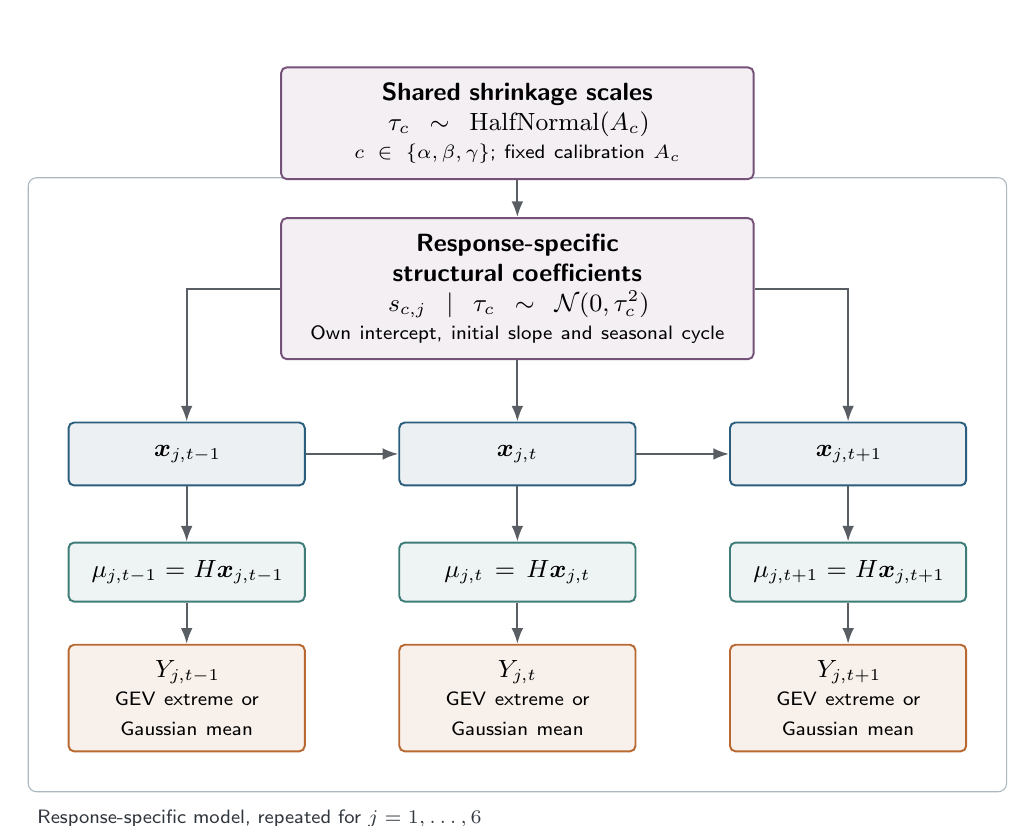
\begin{tikzpicture}[
 font=\sffamily\small,
 box/.style={rounded corners=2pt,draw,line width=.7pt,align=center,
   inner xsep=2mm,inner ysep=2mm},
 state/.style={box,draw=StateBlue,fill=StateBlue!9,text width=2.6cm,minimum height=.8cm},
 location/.style={box,draw=LocationTeal,fill=LocationTeal!9,text width=2.6cm,minimum height=.75cm},
 obs/.style={box,draw=ObservationOrange,fill=ObservationOrange!10,text width=2.6cm,minimum height=1.1cm},
 prior/.style={box,draw=PriorPlum,fill=PriorPlum!9,text width=5.6cm},
 flow/.style={-{Latex[length=2mm]},draw=GraphInk!80,line width=.75pt}
]
 \node[prior] (shared) at (4.2,4.8)
   {\textbf{Shared shrinkage scales}\\
    $\tau_c\sim\operatorname{HalfNormal}(A_c)$\\[-1pt]
    \scriptsize $c\in\{\alpha,\beta,\gamma\}$; fixed calibration $A_c$};
 \node[prior] (coef) at (4.2,2.7)
   {\textbf{Response-specific structural coefficients}\\
    $s_{c,j}\mid\tau_c\sim\mathcal N(0,\tau_c^2)$\\[-1pt]
    \scriptsize Own intercept, initial slope and seasonal cycle};
 \node[state] (xm) at (0,.6) {$\bm x_{j,t-1}$};
 \node[state] (xt) at (4.2,.6) {$\bm x_{j,t}$};
 \node[state] (xp) at (8.4,.6) {$\bm x_{j,t+1}$};
 \node[location] (mm) at (0,-.9) {$\mu_{j,t-1}=H\bm x_{j,t-1}$};
 \node[location] (mt) at (4.2,-.9) {$\mu_{j,t}=H\bm x_{j,t}$};
 \node[location] (mp) at (8.4,-.9) {$\mu_{j,t+1}=H\bm x_{j,t+1}$};
 \node[obs] (ym) at (0,-2.5) {$Y_{j,t-1}$\\[-1pt]\scriptsize GEV extreme or Gaussian mean};
 \node[obs] (yt) at (4.2,-2.5) {$Y_{j,t}$\\[-1pt]\scriptsize GEV extreme or Gaussian mean};
 \node[obs] (yp) at (8.4,-2.5) {$Y_{j,t+1}$\\[-1pt]\scriptsize GEV extreme or Gaussian mean};
 \draw[flow] (shared)--(coef);
 \draw[flow] (coef.south)--(xt.north);
 \draw[flow] (coef.west)-|(xm.north);
 \draw[flow] (coef.east)-|(xp.north);
 \draw[flow] (xm)--(xt);
 \draw[flow] (xt)--(xp);
 \foreach \a/\b in {xm/mm,xt/mt,xp/mp,mm/ym,mt/yt,mp/yp}
   \draw[flow] (\a)--(\b);
 \begin{scope}[on background layer]
  \node[draw=PlateLine,rounded corners=3pt,inner sep=5mm,
    fit=(coef)(xm)(xp)(ym)(yp)] (plate) {};
 \end{scope}
 \node[anchor=north west,font=\sffamily\scriptsize,text=GraphInk]
  at ([yshift=-1mm]plate.south west)
  {Response-specific model, repeated for $j=1,\ldots,6$};
\end{tikzpicture}
\caption{\textbf{Structural model with shared shrinkage.}
Each response has its own level, slope and seasonal state, linked to a
GEV observation distribution for extrema or a Gaussian distribution for
means. Three scales outside the response plate govern the normal priors
on the signed innovation coefficients and are learned from all six
summaries. Their half-normal hyperpriors have fixed calibration scales.
The initial-slope prior remains separately calibrated. Observation
scales and GEV shapes are omitted for clarity.}
\label{fig:state_space_model_structural}
\end{figure}

For summary \(j=1,\ldots,6\), write
\(\bm Y_j=(Y_{j,1},\ldots,Y_{j,T})\),
\(\mathcal X_j=\bm x_{j,0:T}\), and let \(\Theta_j\) contain its
static parameters. With
\(\bm\tau=(\tau_\alpha,\tau_\beta,\tau_\gamma)\), the hierarchical
state-space model factorizes as \citep{sarkka2013}
\begin{equation}\label{eq:ssm}
\begin{aligned}
p(\bm\tau,\Theta,\mathcal X,\bm Y)
&=p(\bm\tau)\prod_{j=1}^{6}
 p(\Theta_j\mid\bm\tau)p(\bm x_{j,0}\mid\Theta_j)\\[-1mm]
&\quad{}\times\prod_{j=1}^{6}\prod_{t=1}^{T}
 p(\bm x_{j,t}\mid\bm x_{j,t-1},\Theta_j)
 g_{j,t}(Y_{j,t}\mid\bm x_{j,t},\Theta_j).
\end{aligned}
\end{equation}
We use a product of the conditional observation likelihoods. Responses
borrow information through the learned prior scales, while retaining
distinct state paths and observation parameters. Conditional on
\(\bm\tau\), their parameter and state priors factorize across responses.
The following subsections specify the states, observations, priors and
computation; the supplement gives the state-space matrices and full target.

	\subsection{State transition}
	\label{subsec::an_interpretable_evolving_location}
	
	Each response has its own level \(\alpha_{j,t}\), slope \(\beta_{j,t}\)
	and dummy-seasonal component \(\gamma_{j,t}\). For seasonal period \(p=4\),
	define
	\begin{equation}\label{eq:state-vector}
		\bm x_{j,t}
		=
		\bigl(
		\alpha_{j,t},\beta_{j,t},
		\gamma_{j,t},\gamma_{j,t-1},\ldots,
		\gamma_{j,t-p+2}
		\bigr)^\top,
		\qquad
		H=(1,0,1,0,\ldots,0).
	\end{equation}
	The state determines the evolving location through
	\begin{equation}\label{eq:location}
		\mu_{j,t}=H\bm x_{j,t}=\alpha_{j,t}+\gamma_{j,t}.
	\end{equation}
	Its components evolve according to
	\begin{subequations}\label{eq:state-transition}
		\begin{align}
			\alpha_{j,t}
			&=\alpha_{j,t-1}+\beta_{j,t-1}
			+s_{\alpha,j}\varepsilon_{\alpha,j,t},
			\label{eq:level}\\
			\beta_{j,t}
			&=\beta_{j,t-1}
			+s_{\beta,j}\varepsilon_{\beta,j,t},
			\label{eq:slope}\\
			\gamma_{j,t}
			&=-\sum_{\ell=1}^{p-1}\gamma_{j,t-\ell}
			+s_{\gamma,j}\varepsilon_{\gamma,j,t}.
			\label{eq:season}
		\end{align}
	\end{subequations}
	The innovations are independent standard normal variables under the state
	prior, and \(q_{c,j}=s_{c,j}^2\) is the process variance of component \(c\).
	
	This local-linear-trend model with stochastic dummy seasonality is a
	standard Bayesian unobserved-components construction
	\citep{harvey1990,west2006,petris2009,scott2014}. The level describes the
	background location, the slope its local rate of change, and the seasonal
	component the departures associated with DJF, MAM, JJA and SON. Small
	innovations allow the trajectory to bend gradually without prespecifying
	changepoints or a spline basis, while keeping observation variability
	separate. As all process variances approach zero, the location reduces to a
	deterministic linear trend plus a fixed seasonal cycle. Interventions,
	additional cycles and external regressors could be included in the same
	framework; we use this parsimonious specification as a starting point for
	nonstationary extremes.
	
	\subsubsection{Non-centred representation}
	\label{subsec::non-centred_representation}
	
	Following \citet{fruhwirthschnatter2010}, we separate each stochastic path from its physical amplitude. The paths have standardized innovations, while signed coefficients determine their contributions to the location. This reduces the tight coupling between paths and process scales near the deterministic limit and makes continuous shrinkage on the amplitudes natural (\cref{subsubsec:shrinkage}).
	
	Let \(\widetilde\alpha_{j,t}\) be a standardized level random walk, \(\widetilde A_{j,t}\) the integrated contribution of a standardized slope random walk, and \(\widetilde\gamma_{j,t}\) a standardized dummy-seasonal process, all initialized at zero. Write \(\gamma^{(0)}_{j,s}\) for the initial seasonal cycle, with \(\sum_{s=1}^{p}\gamma^{(0)}_{j,s}=0\). Then
	\begin{equation}\label{eq:fs}
		\mu_{j,t}
		=\alpha_{j,0}+t\beta_{j,0}+\gamma^{(0)}_{j,s(t)}
		+s_{\alpha,j}\widetilde\alpha_{j,t}
		+s_{\beta,j}\widetilde A_{j,t}
		+s_{\gamma,j}\widetilde\gamma_{j,t}.
	\end{equation}
	The first three terms give a fixed intercept, linear trend and seasonal cycle; the others allow persistent departures from them. The coefficients \(s_{c,j}\) may have either sign, while \(\lvert s_{c,j}\rvert\) is the corresponding innovation standard deviation and \(q_{c,j}=s_{c,j}^2\) its process variance. Conditional on the standardized paths, the signed scales act as regression coefficients. As a scale approaches zero, its path remains well defined and simply contributes less to the location. The reparameterization preserves the state-transition model and its conditional observation likelihood. The standardized recursions and their equivalence to \cref{eq:state-transition} are given in \cref{supp:state-representation}.
	
	\subsection{Observation distributions}
	\label{subsec::observation_distributions}
	
	The state determines the location parameter \(\mu_{j,t}\) of the
	observation distribution. For extrema, this extends the structural
	time-series approach beyond the Gaussian and exponential-family settings
	\citep{helske2017}. In parallel, TXm and TNm are analysed with Gaussian
	observation models:
	\begin{equation}\label{eq:gaussian-observation}
		Y_{j,t}\mid\bm x_{j,t},\Theta_j
		\sim\N(\mu_{j,t},\sigma_{j,t}^2).
	\end{equation}
	TXx and TNx follow the maximum-GEV distribution
	\begin{equation}\label{eq:gev}
		G^+(y;\mu,\sigma,\xi)
		=
		\exp\!\left[
		-\left\{1+\xi\frac{y-\mu}{\sigma}\right\}^{-1/\xi}
		\right],
		\qquad
		1+\xi\frac{y-\mu}{\sigma}>0,
	\end{equation}
	whereas TXn and TNn follow the corresponding minimum-GEV distribution
	\begin{equation}\label{eq:gevmin}
		G^-(y;\mu,\sigma,\xi)
		=
		1-
		\exp\!\left[
		-\left\{1-\xi\frac{y-\mu}{\sigma}\right\}^{-1/\xi}
		\right],
		\qquad
		1-\xi\frac{y-\mu}{\sigma}>0.
	\end{equation}
	The continuous Gumbel limits apply at \(\xi=0\). A negative shape parameter
	implies a finite upper endpoint for a maximum margin and a finite lower
	endpoint for a minimum margin.
	
	The Gaussian and GEV laws are asymptotically motivated observation models
	for block means and extrema. Their limits remain available under suitable
	weak within-block dependence \citep{leadbetter1983}. Serial dependence and
	clustering nevertheless reduce the effective information in a finite block
	and may slow convergence to those limits, so their adequacy is assessed
	empirically.
	
	\subsubsection{Seasonal dispersion}
	\label{subsec:seasonal-dispersion}
	
	In parallel with the fixed seasonal cycle in \cref{eq:fs}, we decompose the
	log observation scale into an overall level and a zero-sum seasonal effect:
	\begin{equation}\label{eq:scale}
		\log\sigma_{j,t}
		=\kappa_j+d_{j,s(t)},
		\qquad
		\sum_{s=1}^{p}d_{j,s}=0.
	\end{equation}
	We enforce the zero-sum constraint through
	\begin{equation}\label{eq:seasonal-scale-coordinates}
		\bm d_j=C_p\bm u_j,
		\qquad C_p^\top C_p=I_{p-1},
		\qquad C_p^\top\bm1_p=\bm0,
	\end{equation}
	where \(\bm d_j=(d_{j,1},\ldots,d_{j,p})^\top\), \(C_p\) is a
	fixed orthonormal contrast matrix, and \(\bm u_j\in\mathbb R^{p-1}\)
	contains the free coefficients. For \(p=4\), three coefficients therefore
	specify the four seasonal log-scale effects.
	Thus \(\exp(\kappa_j)\) is the geometric mean of the four seasonal scales.
	Unlike the evolving seasonal location, the \(d_{j,s}\) are fixed observation
	parameters, so the scale pattern repeats across years. For a Gaussian
	margin, \(\sigma_{j,t}\) is the conditional standard deviation of a seasonal
	mean; for a GEV margin, it is a scale parameter. Neither is the standard
	deviation of daily temperature.
	
	We likewise keep the GEV shape parameter constant and concentrate temporal
	evolution in location, our principal scientific target. The exploratory
	analysis clearly supports seasonal differences in dispersion but not a
	particular secular scale evolution. Time variation in GEV shape is still
	harder to identify because shape is learned from limited tail information
	\citep[Chap.~6]{coles2001}; constant shape is consequently a common
	restriction in nonstationary climate-extreme models \citep{kharin2005}. We
	prespecify this parsimonious model and assess these restrictions using
	period-stratified diagnostics and sensitivity analyses in
	\cref{supp:adequacy}, as well as an outlook for future model selection directions in the Discussion.
	
\subsection{Priors}\label{subsec::priors}

We distinguish uncertainty about the starting state, subsequent climatic
evolution and variability around the latent location. A prior is judged by
what it implies for these quantities in temperature units. Increasing every
prior scale would not provide a neutral default: state innovations
accumulate through time, and a broad prior on a small per-season coefficient
can imply large changes over decades. We therefore calibrate the evolution
priors and examine complete prior simulations
\citep{gelman2017prior,gabry2019}.

For the initial level and the three free coordinates of the initial seasonal
cycle, we retain
\begin{equation}\label{eq:initial-state-priors}
\alpha_{j,0}\sim\N(0,20^2),
\qquad
\bm\gamma^{(0)}_j\sim\N(\bm0,20^2 I_{p-1}).
\end{equation}
These are broad starting-state priors, separate from the priors regulating
subsequent evolution. Their large scale does not establish that the induced
seasonal cycles are physically plausible; this is assessed in
\cref{supp:prior-simulation}. For the observation distributions, we use
\begin{equation}\label{eq:observation-priors}
\exp(2\kappa_j)\sim IG(2,2),
\qquad
\bm u_j\sim\N(\bm0,0.30^2I_{p-1}),
\qquad
\xi_j\sim\N(0,0.30^2).
\end{equation}
Here \(\exp(\kappa_j)\) is the geometric mean of the seasonal observation
scales. The vector \(\bm u_j\) contains their orthonormal log-scale contrast
coordinates: \(\bm d_j=C_p\bm u_j\), as defined in
\cref{eq:seasonal-scale-coordinates}. The shape prior applies only to GEV
margins and is not truncated. The complete specification is given in
\cref{supp:priors}.

\subsubsection{Calibrated hierarchical shrinkage}\label{subsubsec:shrinkage}

In the non-centred representation, the signed innovation coefficients
control departures from a deterministic trend and seasonal cycle. Following
\citet{fruhwirthschnatter2010}, we regularize them towards zero with normal
priors, while estimating their component-specific scales jointly across the
six summaries:
\begin{equation}\label{eq:shrinkage-prior}
\begin{aligned}
s_{c,j}\mid\tau_c&\sim\N(0,\tau_c^2),
&\tau_c&\sim\operatorname{HalfNormal}(A_c),
&&c\in\{\alpha,\beta,\gamma\},\\
\beta_{j,0}&\sim\N(0,P_{\beta_0}).
\end{aligned}
\end{equation}
The half-normal distribution is that of \(A_c|Z|\), where
\(Z\sim\N(0,1)\). Thus \(A_c\) is a fixed calibration scale,
\(\tau_c\) is a learned prior SD, and \(|s_{c,j}|\) is the innovation
SD of response \(j\). The three hyperpriors are independent. Initial
slopes retain separate normal priors with fixed variance \(P_{\beta_0}\).

Sharing \(\tau_c\) lets related summaries inform the typical magnitude of
each kind of evolution while retaining different process variances and
trajectories. It imposes no common warming direction. This is useful when
similar location paths can be obtained by different allocations of level
and slope variation, but it cannot by itself resolve that ambiguity or
ensure prior robustness. Hierarchical scale priors still require calibration
and sensitivity assessment \citep{gelman2006,belmonte2014,bitto2019}.

Our reference calibration is
\begin{equation}\label{eq:shrinkage-prior-scales}
(A_\alpha,A_\beta,A_\gamma)=(10^{-2},10^{-4},10^{-2}),
\qquad P_{\beta_0}=10^{-4}.
\end{equation}
Since \(\E(\tau_c^2)=A_c^2\), the marginal variance of
\(s_{c,j}\) is \(A_c^2\). Over 120 seasonal transitions, the level,
integrated-slope and same-season innovation contributions have prior SDs
of approximately \(0.110\Cdeg\), \(0.075\Cdeg\) and \(0.077\Cdeg\).
The initial-rate prior has SD \(40\sqrt{P_{\beta_0}}=0.40\Cdeg\) per
decade and alone contributes a 30-year displacement SD of \(1.20\Cdeg\).
These scales express a preference for modest changes in evolution, while
allowing uncertainty about a persistent initial rate. They are neither
estimated changes nor upper bounds on warming.

We use ``weakly informative'' to describe the aim of this scientific
calibration, not to claim that the prior has negligible influence on every
latent component. Joint prior simulations include the shared scales,
response-specific coefficients, initial states and observation parameters.
They expose both the implied temperature evolution and the consequences of
the broader starting-state priors. The calculations, simulations and their
limitations are reported in \cref{supp:priors};
\cref{supp:sensitivity} compares scale choices, hyperprior tails and
unpooled formulations.

	\subsection{Posterior computation}\label{sec:posterior_computation}

The conditional structure suggests a blocked Metropolis-within-Gibbs
sampler alternating between response-specific trajectories and parameters,
followed by the shared shrinkage scales \citep{fearnhead_sherlock_2026}.
One sweep of the joint posterior in \cref{eq:ssm} is shown in
\cref{fig:mcmc-sweep}. Given the current shared scales, the six
response-specific blocks can be updated in parallel; the scales are then
updated using all six coefficient sets.

\begin{figure}[!htbp]
\centering
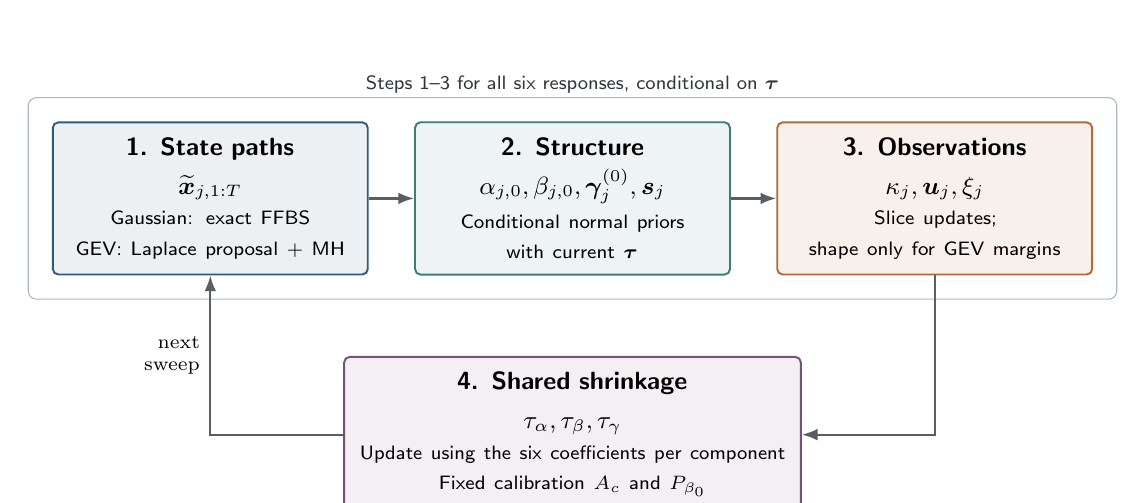
\begin{tikzpicture}[
 font=\sffamily\small,
 block/.style={rounded corners=2pt,text width=3.6cm,minimum height=1.85cm,
   align=center,inner sep=2mm,line width=.7pt},
 stateblock/.style={block,draw=StateBlue,fill=StateBlue!9},
 coefblock/.style={block,draw=LocationTeal,fill=LocationTeal!9},
 obsblock/.style={block,draw=ObservationOrange,fill=ObservationOrange!10},
 hyperblock/.style={block,draw=PriorPlum,fill=PriorPlum!9,text width=5.4cm},
 flow/.style={-{Latex[length=2mm]},draw=GraphInk!80,line width=.8pt}
]
 \node[stateblock] (path) at (0,0) {\textbf{1. State paths}\\[3pt]
   $\widetilde{\bm x}_{j,1:T}$\\[3pt]
   \scriptsize Gaussian: exact FFBS\\GEV: Laplace proposal + MH};
 \node[coefblock] (coef) at (4.6,0) {\textbf{2. Structure}\\[3pt]
   $\alpha_{j,0},\beta_{j,0},\bm\gamma^{(0)}_j,\bm s_j$\\[3pt]
   \scriptsize Conditional normal priors\\with current $\bm\tau$};
 \node[obsblock] (obs) at (9.2,0) {\textbf{3. Observations}\\[3pt]
   $\kappa_j,\bm u_j,\xi_j$\\[3pt]
   \scriptsize Slice updates;\\shape only for GEV margins};
 \draw[flow] (path)--(coef);
 \draw[flow] (coef)--(obs);
 \begin{scope}[on background layer]
  \node[draw=PlateLine,rounded corners=3pt,inner sep=3mm,
    fit=(path)(coef)(obs)] (plate) {};
 \end{scope}
 \node[font=\scriptsize\sffamily,text=GraphInk,align=center]
   at (4.6,1.45) {Steps 1--3 for all six responses, conditional on $\bm\tau$};
 \node[hyperblock] (hyper) at (4.6,-3.0)
   {\textbf{4. Shared shrinkage}\\[3pt]
    $\tau_\alpha,\tau_\beta,\tau_\gamma$\\[3pt]
    \scriptsize Update using the six coefficients per component\\
    Fixed calibration $A_c$ and $P_{\beta_0}$};
 \draw[flow] (obs.south)--(9.2,-3.0)--(hyper.east);
 \draw[flow] (hyper.west)--(0,-3.0)--
   node[left,font=\scriptsize,align=right]{next\\sweep}(path.south);
\end{tikzpicture}
\caption{\textbf{One sweep of the hierarchical posterior sampler.}
The response-specific path, structural and observation updates are
conditional on the current shared scales. A fourth block updates the
three shrinkage scales from all six responses. The half-normal calibration
scales and initial-slope prior variance stay fixed. Gaussian paths use
exact FFBS; GEV paths use a Laplace proposal with an exact MH correction.
Independent MCMC chains target the complete hierarchy.}
\label{fig:mcmc-sweep}
\end{figure}

	For a Gaussian response, the observation equation is linear in the
	standardized states when the structural coefficients are held fixed. The
	complete path can therefore be sampled exactly by forward filtering and
	backward sampling (FFBS) \citep{carter1994,fruhwirthschnatter1994,durbin2000,durbin2012}.
	For a GEV margin, a local Laplace approximation \(\widetilde L\) to the exact
	conditional likelihood \(L\) defines the independence proposal
	\begin{equation}\label{eq:gev-path-proposal}
		q(\widetilde{\bm x}_j)
		\propto
		p_0(\widetilde{\bm x}_j)\widetilde L(\widetilde{\bm x}_j),
	\end{equation}
	which is sampled by FFBS. A proposed complete path
	\(\widetilde{\bm x}_j^\star\) is accepted with probability
	\begin{equation}\label{eq:mh}
		\rho_{\mathrm{MH}}
		(\widetilde{\bm x}_j,\widetilde{\bm x}_j^\star)
		=
		\min\!\left\{
		1,
		\frac{
			L(\widetilde{\bm x}_j^\star)\widetilde L(\widetilde{\bm x}_j)
		}{
			L(\widetilde{\bm x}_j)\widetilde L(\widetilde{\bm x}_j^\star)
		}
		\right\}.
	\end{equation}
	The approximation is held fixed during this update. Because \(L\) includes
	the exact GEV density and support, the correction preserves the
	specified conditional posterior; approximation quality affects efficiency,
	not the retained target.
	
	Conditional on the paths, Gaussian structural coefficients have direct
	Gaussian updates, whereas GEV coefficient blocks use elliptical slice
	sampling with an exact conditional target \citep{murray2010}. The remaining
	observation parameters are updated by elliptical
	or componentwise stepping-out slice sampling as appropriate \citep{neal2003}.
	The shared shrinkage scales have one-dimensional full conditionals and
are updated on the log scale. The complete target, Gaussian state update,
proposal construction and shrinkage update are given in \cref{supp:computation}.
	
	\section{Model assessment and predictive performance}
	\label{sec::goodness-of-fit}
	
	We first assess marginal fit using probability integral transform
	(PIT) histograms and normal-score Q--Q plots. For the conditional CDF
	\(G_{j,t}\) on the original temperature scale, define
	\begin{equation}\label{eq:pit-scores}
		U_{j,t}=G_{j,t}(Y_{j,t}\mid\bm x_{j,t},\Theta_j),
		\qquad Z_{j,t}=\Phi^{-1}(U_{j,t}),
	\end{equation}
	where \(\Phi\) is the standard-normal CDF. Correctly specified continuous
	conditional margins give the reference distributions
	\begin{equation}\label{eq:pit-reference}
		U_{j,t}\sim\operatorname{Unif}(0,1),
		\qquad Z_{j,t}\sim\N(0,1).
	\end{equation}
	PITs computed from posterior-smoothed states reuse the fitted observations
	and are descriptive residual diagnostics rather than calibrated forecasts.
	Posterior predictive checks compare observed normal-score dispersion,
	skewness and tail frequencies with those of replicated scores under the
	same posterior draws \citep{gelman1996}. Details are given in
	\cref{supp:adequacy}.
	
	Forecasting follows directly from the state equations. Conditional
	on a posterior draw of the terminal state and parameters, the mean
	forecast of the latent location \(h\) seasons ahead is
	\begin{equation}\label{eq:forecast-location}
		\mu_{j,T+h\mid T}
		=\alpha_{j,T}+h\beta_{j,T}+\gamma_{j,T+h\mid T}.
	\end{equation}
	Here \(\gamma_{j,T+h\mid T}\) is the seasonal component forecast from
	the state at \(T\), obtained by propagating the dummy-seasonal
	transition with future innovations set to zero. The implied cycle
	repeats every four seasons. Full predictive simulations instead draw
	future innovations and then Gaussian or GEV observations, propagating
	uncertainty in the terminal state, parameters and future evolution
	together with observation variability. \Cref{supp:risk} gives the
	forecast calculations.
	
	We assess predictive performance through expanding-window refits,
	using only observations of all six summaries available at each forecast
origin; the shared scales are re-estimated within each training window. Forecast
	calibration is examined using PIT plots and the coverage and average
	width of central \(90\%\), \(95\%\) and \(99\%\) prediction intervals.
	Predictive accuracy is compared using CRPS, with smaller values
	indicating better performance \citep{diebold1998,gneiting2007}.
	The forecast design, seasonal breakdowns and directional tail misses
	are reported in \cref{supp:adequacy}.
	
	\section{Tracking evolving risk}\label{sec:tracking-risk}
	
	The fitted distributions describe both the rarity of a fixed
	temperature and the temperature associated with a fixed rarity.
	For the seasonal CDF \(G_{j,t}\), upper- and lower-tail probabilities are
	\begin{equation}\label{eq:threshold-risk}
		p^+_{j,t}(c)=1-G_{j,t}(c),
		\qquad
		p^-_{j,t}(c)=G_{j,t}(c).
	\end{equation}
	For example, the upper-tail probability for JJA TXx describes the
	chance of at least one summer day exceeding \(c\). For a specified
	season, \(\mathcal R^\pm_{j,t}(c)=1/p^\pm_{j,t}(c)\) is its
	stationary-equivalent return period in years. This describes
	recurrence if that season's distribution remained unchanged, rather
	than the expected waiting time under an evolving climate
	\citep{cooley2012,salas2014}. Conversely, the upper- and lower-tail
	\(r\)-year return levels, for \(r>1\), are the quantiles
	\begin{equation}\label{eq:seasonal-return-levels}
		z^+_{j,t}(r)=G_{j,t}^{-1}(1-1/r),
		\qquad
		z^-_{j,t}(r)=G_{j,t}^{-1}(1/r).
	\end{equation}
	We calculate these quantities within each posterior draw and report
	medians and pointwise 95\% credible intervals. The simulated future
	paths from \cref{sec::goodness-of-fit} extend the same calculations
	to forecasts of return periods and levels; averaging the conditional
	exceedance probabilities gives the predictive event probability.
	
	Calculations for annual summaries and risks over longer forecast
	windows are given in \cref{supp:risk}.
	
	% Editorial note: the Results section below is preserved verbatim from the supplied draft.
% Its numbers, figures and pending-fit labels must be refreshed after the hierarchical runs.
% They are not newly computed half-normal-hierarchy results.
	% Historical-contrast results and the historical-fit appendix have been removed.
	\section{Results}\label{sec:results}
	
	\begin{resultbox}{Computation: update from the separate fits}
		Insert the completed-run chain lengths, convergence summaries and
		computational cost. The screen and paper settings are specified in
		\cref{supp:sensitivity}; report the settings of the actual fits used
		for the numerical results.
	\end{resultbox}
	
	The whole-path proposals were highly efficient: GEV paths were accepted
	in 97.2\% of updates overall, ranging from 95.2\% for TNn to 98.6\% for
	TXn. This high acceptance rate indicates that the Gaussian state-space
	proposal closely approximated the exact conditional target. Every local
	optimization used to construct a proposal converged, and no proposal was
	rejected because the optimizer failed to respect the GEV support.
	
	
	The posterior GEV shape medians were \(-0.190\) for TXx, \(-0.230\) for
	TXn, \(-0.156\) for TNx and \(-0.116\) for TNn, with respective 95\%
	credible intervals \((-0.234,-0.141)\), \((-0.275,-0.182)\),
	\((-0.199,-0.108)\) and \((-0.165,-0.061)\). All four relevant tails are
	therefore estimated to be bounded, having finite statistical
	endpoints. Trace plots, Monte Carlo errors (rank-normalized splits and effective sample sizes) and sensitivity checks are
	provided in \cref{supp:adequacy,supp:sensitivity}.
	
	Seasonal dispersion is clearly response-specific (\cref{fig:seasonal-scales}). DJF has the largest median scale for TXm and TNm (\(1.45\Cdeg\) and \(1.46\Cdeg\)), and TNm falls to \(0.68\Cdeg\) in JJA. Among the extrema, TXx is most dispersed in SON (\(2.70\Cdeg\)), whereas TXn and TNn are again most dispersed in DJF (\(2.78\Cdeg\) and \(3.05\Cdeg\)). Separating this important recurring pattern from the latent location prevents the state evolution from having to reproduce predictable changes in spread.
	
	\paperfigure{seasonal_scales.png}{0.98}{\textbf{Seasonal observation scales.}
		Points and bars show posterior medians and 95\% credible intervals; small horizontal offsets separate the summaries. For TXm and TNm, scale is the conditional standard deviation of a seasonal mean. For the extrema it is the GEV scale parameter, not a standard deviation.}{fig:seasonal-scales}
	
	The pooled PIT histograms and normal-score Q--Q plots are broadly consistent with their reference distributions (\cref{fig:seasonal-pit}). The clearest feature is mild left-skewness in the TNm normal scores. Two-sided Kolmogorov--Smirnov tests likewise provide no evidence against uniformity, with \(p\)-values of \(0.578\) (TXm), \(0.107\) (TNm), \(0.948\) (TXx), \(0.929\) (TXn), \(0.619\) (TNx) and \(0.711\) (TNn). Because the PITs are obtained in-sample and retain some serial dependence, these tests are interpreted descriptively. Season-stratified diagnostics in Supplementary \ref{supp:adequacy} reveal several localized departures that are obscured by pooling and examine the remaining serial structure.
	
	\paperfigure{seasonal_pit_qq.png}{1}{\textbf{Goodness-of-fit diagnostics.} For each response, the dashed line indicates the uniform-density reference. The corresponding Q--Q plot compares normal-score-transformed PITs with standard-normal quantiles. These are in-sample diagnostics; season-stratified versions are provided in Supplementary \cref{supp:adequacy}.}{fig:seasonal-pit}
	
	\begin{resultbox}{Prior sensitivity: screen results pending}
		The complete settings and figure placeholders are in
		\cref{supp:sensitivity}. Insert the main findings on levels, warming rates,
		seasonal evolution and risk probabilities after checking the separate fits.
	\end{resultbox}
	
	
	Expressed on a ten-year horizon, the posterior median standard deviations generated by new level innovations range from \(0.085\Cdeg\) to \(0.195\Cdeg\) for the different summaries, those generated by accumulated slope innovations from \(0.035\Cdeg\) to \(0.048\Cdeg\), and those generated by same-season innovations from \(0.016\Cdeg\) to \(0.046\Cdeg\). These quantities describe the stochastic contribution of the state innovations. Their magnitude permits gradual changes in the latent trajectories without allowing them to follow short-term seasonal weather noise.
	
	\subsection{Evolution of levels and warming rates}
	\label{subsec:historical-change}
	
	All six fitted levels rise across the record
	(\cref{fig:seasonal-levels}). Daytime trajectories flatten or dip around
	mid-century before rising more strongly from the 1970s, whereas nighttime
	trajectories increase more steadily.
	
	\paperfigure{seasonal_levels.png}{0.98}{\textbf{Latent temperature levels,
			1892--2026.} Curves and bands show posterior medians and pointwise 95\%
		credible intervals for TX summaries (top row) and TN summaries (bottom
		row), in the original temperature orientation.}{fig:seasonal-levels}
	
	The slope trajectories describe the local rate of change
	(\cref{fig:seasonal-slopes}). Their posterior bands show uncertainty in
	when and how quickly the fitted levels change, particularly near the
	ends of the record. Sensitivity to the structural priors is examined in
	\cref{supp:sensitivity}.
	
	\paperfigure{seasonal_slopes.png}{0.98}{\textbf{Local warming rates.}
		Curves and bands show posterior medians and pointwise 95\% credible
		intervals in degrees Celsius per decade, in the original temperature
		orientation. Dashed lines mark zero.}{fig:seasonal-slopes}
	
	\FloatBarrier
	
	\subsection{Evolving risk and prediction}
	The location shifts translate nonlinearly into event probabilities (\cref{fig:seasonal-risks}).
	For JJA, the posterior median probability that TXx exceeds \(35\Cdeg\) rises from 3.6\% (95\% interval 1.7--6.7\%) in the first 30 years of the record to 15.9\% (11.1--22.0\%) in the most recent 30 years and 22.4\% (14.2--34.0\%) in 2026 . Under conditions held fixed at each of those periods, that would correspond to roughly one summer in 28, one in six and one in four/five.
	
	\paperfigure{seasonal_risks.png}{0.96}{\textbf{Changing seasonal risks.} Posterior median event probabilities and pointwise 95\% credible intervals for JJA TXx \(>35\Cdeg\), JJA TNx \(>25\Cdeg\), DJF TXn \(<0\Cdeg\) and DJF TNn \(<-10\Cdeg\).}{fig:seasonal-risks}
	
	The chance of a summer containing a daily minimum above \(25\Cdeg\) also rises, although such a hot night remains unusual: the fitted JJA probability increases from 0.0024\% (0--0.072\%) in the early period to 0.186\% (0.024--0.742\%) recently and 0.377\% (0.061--1.331\%) in 2026. At the cold end, a winter containing an \textit{ice day}—a day whose maximum stays below \(0\Cdeg\)—becomes somewhat less likely: its probability falls from 94.7\% (90.9--97.2\%) to 79.5\% (72.8--85.3\%). The probability of a winter minimum below \(-10\Cdeg\) falls from 45.8\% (38.1--54.5\%) to 25.8\% (19.5--32.6\%). For DJF 2026, the corresponding fitted probabilities are 73.3\% and 21.3\%.
	
	Uccle's reported heat record of \(36.6\Cdeg\), set in 1947, stood for 72 years. By spring 2019, a new record was plausible. Fitted using observations only through May 2019, the model assigned the coming summer an 11.5\% probability of exceeding \(35\Cdeg\) (6.5--18.2\%) and a 3.1\% probability of exceeding the old record (1.1--6.3\% \cref{fig:pre2019-record}).
	
	The summer that followed was exceptionally hot. On 25 July, Uccle reached \(39.7\Cdeg\), surpassing the 1947 benchmark by \(3.1\Cdeg\). Before the season, the fitted probability of an extreme this high was only 0.046\%---about 70 times smaller than the probability of breaking the old record. The posterior median conditional probability was 0.016\% (95\% interval 0--0.265\%). This was a record-shattering extreme \citep{fischer2025}.
	
	The heat extended beyond that single daytime maximum: all six observed JJA 2019 summaries exceeded their predictive medians, while TXx and TNx also exceeded the upper limits of their 95\% prediction intervals. 
	
	
	\paperfigure{pre2019_record_event.png}{1}{\textbf{The 2019 record summer viewed from May 2019.} \emph{A:} One-season-ahead predictive medians and 95\% prediction intervals for the six JJA summaries; diamonds show the observations. \emph{B:} Posterior mean probability of JJA TXx exceeding each threshold, with pointwise 95\% intervals for the conditional probability. The gold point marks \(35\Cdeg\); the red point and vertical line mark the observed \(39.7\Cdeg\).}{fig:pre2019-record}
	
	
	Ten-year forecasts propagate the terminal posterior state through the same structural evolution used within the observed period. Their central tendency continues the latest estimated local trend, while future state innovations allow individual trajectories to depart from that extrapolation. These are statistical forecasts rather than climate projections and are not conditioned on a particular emissions scenario. For JJA 2036, the posterior median probability that TXx exceeds \(35\Cdeg\) is \(26.9\%\) (\(14.9\%--46.5\%\)), while the probability that TNx exceeds \(25\Cdeg\) is \(0.58\%\) (\(0.09\%--2.49\%\)). For DJF 2036, the probabilities that TXn falls below \(0\Cdeg\) and TNn below \(-10\Cdeg\) are \(68.8\%\) (\(54.4\%--80.6\%\)) and \(18.9\%\) (\(11.7\%--27.5\%\)), respectively. These intervals propagate uncertainty in the terminal state and model parameters together with future state innovations.
	
	It is important to distinguish uncertainty about the latent climate state from the variability of a future observation. In \cref{fig:forecast-uncertainty}, the 95\% prediction intervals for future JJA TXm and TXx observations are substantially wider than the corresponding posterior intervals for their latent locations. For TXx, the GEV location parameter is moreover not the predictive median: \(G^+(\mu)=\exp(-1)\), so \(\mu\) represents approximately the 37th percentile of a (maximum) GEV distribution.
	
	The gradual widening of the forecast bands follows from the state transition. Isolating the level and slope innovations, their contribution at a horizon of \(h\) seasonal blocks is
	\begin{equation}\label{eq:forecastvariance}
		\operatorname{Var}\!\left(
		\alpha_{j,T+h}\mid
		\alpha_{j,T},\beta_{j,T},\Theta_j
		\right)
		=
		h s_{\alpha,j}^{2}
		+
		s_{\beta,j}^{2}
		\frac{h(h-1)(2h-1)}{6}.
	\end{equation}
	Although this uncertainty accumulates with the forecast horizon, the estimated innovation scales are small. Over ten years, its contribution is therefore modest relative to the much larger interannual observation variability, whose season-specific scale does not itself increase with the horizon.
	
	\textbf{The present ten-year display does not yet show the accumulation of state uncertainty sufficiently clearly, because its contribution remains small relative to ordinary weather variability. We will therefore replace it with a 30-year forecast display, directly addressing the reviewer’s question of how predictive uncertainty broadens with the forecast horizon.}
	
	\paperfigure{forecast_uncertainty_seasonal.png}{0.98}{\textbf{Ten-year JJA temperature forecasts.} Top: 95\% prediction intervals for future TXm and TXx observations (blue) and 95\% posterior intervals for their latent locations (red), 2027--2036. Bottom: widths of the corresponding intervals.}{fig:forecast-uncertainty}
	
	
	\section{Discussion}\label{sec:discussion}
	
	Structural time-series models give an extreme-value distribution an
	interpretable changing history. The latent level, slope and seasonal cycle
	describe persistent evolution, while the observation distribution accounts
	for variability among seasonal summaries. In the Uccle application,
	cumulative warming is clearer than the detailed history of changes in its
	rate, particularly near the record boundaries. This distinction matters:
	a smooth fitted trajectory need not imply a precisely estimated local rate,
	and its bends do not identify physical causes.
	
	The methodological challenge is learning how strongly the latent components
	should evolve. Small innovations can have substantial cumulative effects
	while remaining weakly informed by individual observations. The non-centred
representation makes their amplitudes accessible to continuous shrinkage.
The sensitivity of the preliminary single-series fits motivated a further
step: pooling the strength of regularization across related summaries.
A long record can constrain the overall location while leaving substantial
ambiguity about how level and slope innovations produce it. Each fitted
rate can then depend strongly on the separately chosen prior scales.

The hierarchy lets all six summaries inform three component-specific
shrinkage scales and may stabilize the allocation of variation while
preserving distinct histories. Whether it achieves this must be established
by the sensitivity comparisons; partial pooling is not a guarantee of
identification. Its
scientific value is reduced sensitivity of the posterior trajectories and
risk estimates, rather than narrower intervals by themselves. The unpooled
comparisons in \cref{supp:unpooled} and the alternative hyperpriors in
\cref{supp:hyperprior-families} assess this benefit. Only six coefficients
inform each shared scale, so borrowing information complements physical
calibration and sensitivity assessment; it does not remove their need.
Stable level estimates may still coexist with uncertainty about local
rates or seasonal evolution.

Calibration gives these priors a scientific interpretation. The same numerical
scale can imply very different temperature changes for a level random walk,
an integrated slope or a seasonal component. Weak informativeness therefore
concerns their implications within the model, not the number of decimal
places in a coefficient or an arbitrarily large prior variance
\citep{gelman2017prior,gabry2019}. The reference favours modest departures
from a persistent trend and seasonal cycle; the sensitivity analysis tests
whether the resulting trajectories and risks depend materially on that
preference. Hyperpriors extend this calibration by allowing the responses
to learn common evolution scales, while their tail behaviour remains an
explicit modelling choice \citep{gelman2006}.

The joint prior simulations also reveal a limitation of the retained
starting-state specification. The SD-20 seasonal-coordinate priors generate
very broad annual cycles and substantial mass on implausible temperature
patterns. This finding is separate from the much smaller prior changes in
seasonality over 30 years. It motivates assessing a tighter, physically
interpretable initial-cycle prior, including its coordinate dependence,
rather than broadening stochastic evolution scales to address every source
of sensitivity. The current simulations provide a diagnostic of the stated
model; they do not certify all of its priors as weakly informative or make
its six replicated summaries physically ordered.
	
	The state update exploits the latent Gaussian structure while retaining the
	GEV observation law. Gaussian simulation smoothing supplies a complete-path
	proposal, and the Metropolis--Hastings correction preserves the posterior
	target. High acceptance in the present application supports the usefulness
	of this proposal; it does not replace convergence checks or establish its
	efficiency for every extreme-value likelihood. Comparisons with particle
	MCMC would help determine how performance changes with stronger nonlinearities,
	longer records or observations close to finite endpoints
	\citep{andrieu2010,lindsten2014}.
	
	The risk calculations connect distributional evolution to events with a
	direct temperature interpretation. A familiar threshold can become much more
	likely while an extreme overshoot remains exceptional, as illustrated by
	the 2019 summer \citep{fischer2025}. Return periods must therefore be read
	as stationary equivalents of the fitted seasonal probabilities. Forecasts
	propagate uncertainty in the current state and subsequent evolution, but
	extrapolate statistical dynamics rather than an emissions scenario.
	
	The summaries are derived from the same days and are likely to retain
positive residual correlations, especially between daytime and nighttime
temperatures. Sharing prior scales does not represent this residual
association. Our product of conditional observation likelihoods is therefore
a working assumption whose effect on the uncertainty of pooled estimates
requires assessment. A richer observation model would also be needed for
formal contrasts between summaries, since uncertainty in a difference
depends on their covariance. Overlap of marginal credible intervals cannot
establish equal warming.
	
	Several modelling restrictions warrant further assessment. Observation
	scales repeat by season, and the GEV shapes are constant through time.
	Changes in these features may matter for remote thresholds even when the
	location describes most historical variation. Seasonal maxima also do not
	describe the duration or clustering of heatwaves. Prior sensitivity,
	posterior predictive checks and held-out forecasts address different parts
	of model adequacy; none alone establishes reliable extrapolation far beyond
	the observed range.
	
	Continuous shrinkage also leaves open which components should evolve at
	all \citep{slater2020}. It allows innovation scales arbitrarily close to
	zero without assigning probability to an exactly fixed component. Formal
	selection between fixed and evolving levels, slopes or seasonal cycles
	would require a separate model-selection construction, for example point
	masses or dimension-changing moves
	\citep{fruhwirthschnatter2010,cadonna2020,green1995}. Near the deterministic
	limit, such procedures must distinguish absent evolution from evolution
	too weak to detect, and should be judged through their effects on the
	scientific quantities of interest.
	
	The framework can be adapted to other environmental variables whose
	distributional features evolve. Hydrological extremes
	\citep{katz2002} and precipitation applications may require changing
	occurrence, scale or shape alongside location
	\citep{asadieh2015,westra2013,bhatia2019,gu2017,jorgensen2024,jayaweera2025,razighalavand2025}.
	Snow loads and wave climates provide further applications
	\citep{leroux2022,wang2004}, while drought requires particular attention
	to persistence and accumulation \citep{vanloon2015}. An \(r\)-largest
	analysis could use more than one extreme per block; threshold and runs
	models could address event clustering and duration \citep{coles2001}.
	Additional sites or physical covariates could provide regional context
	\citep{scott2014}. Each extension calls for suitable observation and state
	components, renewed prior calibration and predictive validation.
	
	\section{Conclusion}\label{sec:conclusion}
	
	Bayesian structural models make evolving environmental risks estimable
	while learning the strength of persistent change. Combining interpretable
	latent components, calibrated hierarchical shrinkage and an exact
correction to Gaussian state proposals provides a practical framework for
extremes, with Gaussian models for averages considered alongside them.
Related responses inform the regularization while retaining their own
trajectories. Analytic calibration and joint prior simulation make the
implied magnitudes of evolution explicit and distinguish them from broad
uncertainty about the starting state. The Belgian temperature application illustrates how the
framework tracks
	warming and changing threshold probabilities while representing uncertainty
	in local rates and future conditions. Extensions to other hazards and to
	selection of the evolving components offer further opportunities for
	state-space extreme-value analysis.
	
	\FloatBarrier
	
	\begin{thebibliography}{115}
		\small
		\setlength{\itemsep}{2pt}
		
		\bibitem[Alexander et al.(2006)]{alexander2006}
		Alexander, L.V., Zhang, X., Peterson, T.C., Caesar, J., Gleason, B., Klein Tank, A., Haylock, M., Collins, D., Trewin, B., Rahimzadeh, F., et al.: Global observed changes in daily climate extremes of temperature and precipitation. Journal of Geophysical Research: Atmospheres 111(D5) (2006)
		
		\bibitem[Alexander(2016)]{alexander2016}
		Alexander, L.V.: Global observed long-term changes in temperature and precipitation extremes: A review of progress and limitations in IPCC assessments and beyond. Weather and Climate Extremes 11, 4--16 (2016)
		
		\bibitem[Andrieu et al.(2010)]{andrieu2010}
		Andrieu, C., Doucet, A., Holenstein, R.: Particle Markov chain Monte Carlo methods. Journal of the Royal Statistical Society Series B: Statistical Methodology 72(3), 269--342 (2010)
		
		\bibitem[Asadieh and Krakauer(2015)]{asadieh2015}
		Asadieh, B., Krakauer, N.Y.: Global trends in extreme precipitation: climate models versus observations. Hydrology and Earth System Sciences 19(2), 877--891 (2015)
		
		\bibitem[Beaulieu et al.(2012)]{beaulieu2012}
		Beaulieu, C., Chen, J., Sarmiento, J.L.: Change-point analysis as a tool to detect abrupt climate variations. Phil. Trans. R. Soc. A 370(1962), 1228--1249 (2012) \url{https://doi.org/10.1098/rsta.2011.0383}
		
		\bibitem[Beaulieu et al.(2024)]{beaulieu2024}
		Beaulieu, C., Gallagher, C., Killick, R., Lund, R., Shi, X.: A recent surge in global warming is not detectable yet. Commun Earth Environ 5(1), 576 (2024) \url{https://doi.org/10.1038/s43247-024-01711-1}
		
		\bibitem[Belmonte et al.(2014)]{belmonte2014}
		Belmonte, M.A., Koop, G., Korobilis, D.: Hierarchical shrinkage in time-varying parameter models. Journal of Forecasting 33(1), 80--94 (2014)
		
		\bibitem[Bhatia and Ganguly(2019)]{bhatia2019}
		Bhatia, U., Ganguly, A.R.: Precipitation extremes and depth-duration-frequency under internal climate variability. Scientific reports 9(1), 9112 (2019)
		
		\bibitem[Bitto and Frühwirth-Schnatter(2019)]{bitto2019}
		Bitto, A., Frühwirth-Schnatter, S.: Achieving shrinkage in a time-varying parameter model framework. Journal of Econometrics 210(1), 75--97 (2019)
		
		\bibitem[Brown et al.(2008)]{brown2008}
		Brown, S.J., Caesar, J., Ferro, C.A.T.: Global changes in extreme daily temperature since 1950. Journal of Geophysical Research 113, D05115 (2008). \url{https://doi.org/10.1029/2006JD008091}
		
		\bibitem[Bürkner et al.(2020)]{burkner2020}
		Bürkner, P.-C., Gabry, J., Vehtari, A.: Approximate leave-future-out cross-validation for Bayesian time series models. Journal of Statistical Computation and Simulation 90(14), 2499--2523 (2020). \url{https://doi.org/10.1080/00949655.2020.1783262}
		
		\bibitem[Cadonna et al.(2020)]{cadonna2020}
		Cadonna, A., Frühwirth-Schnatter, S., Knaus, P.: Triple the gamma---a unifying shrinkage prior for variance and variable selection in sparse state space and tvp models. Econometrics 8(2), 20 (2020)
		
		\bibitem[Cahill et al.(2015)]{cahill2015}
		Cahill, N., Rahmstorf, S., Parnell, A.C.: Change points of global temperature. Environ. Res. Lett. 10(8), 084002 (2015) \url{https://doi.org/10.1088/1748-9326/10/8/084002}
		
		\bibitem[Carlin et al.(1992)]{carlin1992}
		Carlin, B.P., Polson, N.G., Stoffer, D.S.: A Monte Carlo approach to nonnormal and nonlinear state-space modeling. Journal of the american Statistical association 87(418), 493--500 (1992)
		
		\bibitem[Caroni and Panagoulia(2016)]{caroni2016}
		Caroni, C., Panagoulia, D.: Non-stationary modelling of extreme temperatures in a mountainous area of greece. REVSTAT-Statistical Journal 14(2), 217--228 (2016)
		
		\bibitem[Carter and Kohn(1994)]{carter1994}
		Carter, C.K., Kohn, R.: On Gibbs sampling for state space models. Biometrika 81(3), 541--553 (1994)
		
		\bibitem[Cheng et al.(2014)]{cheng2014}
		Cheng, L., AghaKouchak, A., Gilleland, E., Katz, R.W.: Non-stationary extreme value analysis in a changing climate. Climatic change 127, 353--369 (2014) \url{https://doi.org/10.1007/s10584-014-1254-5}
		
		\bibitem[Carvalho et al.(2009)]{carvalho2009}
		Carvalho, C.M., Polson, N.G., Scott, J.G.: Handling sparsity via the horseshoe. Artificial intelligence and statistics, 73--80 (2009)
		
		\bibitem[Chernozhukov et al.(2017)]{chernozhukov2017}
		Chernozhukov, V., Fernández-Val, I., Kaji, T.: Extremal quantile regression. Handbook of Quantile Regression, 333--362 (2017)
		
		\bibitem[Coles(2001)]{coles2001}
		Coles, S.: An Introduction to Statistical Modeling of Extreme Values. Springer, London (2001). \url{https://doi.org/10.1007/978-1-4471-3675-0}
		
		\bibitem[Contzen et al.(2023)]{contzen2023}
		Contzen, J., Dickhaus, T., Lohmann, G.: Long-term temporal evolution of extreme temperature in a warming earth. Plos one 18(2), 0280503 (2023)
		
		\bibitem[Cooley(2012)]{cooley2012}
		Cooley, D.: Return periods and return levels under climate change. in: Extremes in a changing climate. Water Science and Technology Library 65, 97--114 (2012) \url{https://doi.org/10.1007/978-94-007-4479-0_4}
		
		\bibitem[Coumou et al.(2013)]{coumou2013}
		Coumou, D., Robinson, A., Rahmstorf, S.: Global increase in record-breaking monthly-mean temperatures. Climatic Change 118(3), 771--782 (2013)
		
		\bibitem[Davison and Ramesh(2000)]{davison2000}
		Davison, A.C., Ramesh, N.I.: Local likelihood smoothing of sample extremes. Journal of the Royal Statistical Society: Series B (Statistical Methodology) 62(1), 191--208 (2000). \url{https://doi.org/10.1111/1467-9868.00228}
		
		\bibitem[Donat and Alexander(2012)]{donat2012}
		Donat, M.G., Alexander, L.V.: The shifting probability distribution of global daytime and night-time temperatures. Geophys. Res. Lett. 39(14) (2012) \url{https://doi.org/10.1029/2012GL052459}
		
		\bibitem[Donat et al.(2013)]{donat2013}
		Donat, M., Alexander, L.V., Yang, H., Durre, I., Vose, R., Dunn, R.J., Willett, K.M., Aguilar, E., Brunet, M., Caesar, J., et al.: Updated analyses of temperature and precipitation extreme indices since the beginning of the twentieth century: The hadex2 dataset. J. Geophys. Res. Atmos 118(5), 2098--2118 (2013) \url{https://doi.org/10.1002/jgrd.50150}
		
		\bibitem[Dunn et al.(2019)]{dunn2019}
		Dunn, R.J., Willett, K.M., Parker, D.E.: Changes in statistical distributions of subdaily surface temperatures and wind speed. Earth System Dynamics 10(4), 765--788 (2019)
		
		\bibitem[Durbin and Koopman(2000)]{durbin2000}
		Durbin, J., Koopman, S.J.: Time series analysis of non-Gaussian observations based on state space models from both classical and Bayesian perspectives. Journal of the Royal Statistical Society Series B: Statistical Methodology 62(1), 3--56 (2000)
		
		\bibitem[Durbin and Koopman(2012)]{durbin2012}
		Durbin, J., Koopman, S.J.: Time Series Analysis by State Space Methods. Oxford University Press, Oxford (2012)
		
		\bibitem[Easterling et al.(2000)]{easterling2000}
		Easterling, D.R., Meehl, G.A., Parmesan, C., Changnon, S.A., Karl, T.R., Mearns, L.O.: Climate extremes: observations, modeling, and impacts. Science 289(5487), 2068--2074 (2000) \url{https://doi.org/10.1126/science.289.5487.2068}
		
		\bibitem[Easterling et al.(2016)]{easterling2016}
		Easterling, D.R., Kunkel, K.E., Wehner, M.F., Sun, L.: Detection and attribution of climate extremes in the observed record. Weather and Climate Extremes 11, 17--27 (2016)
		
		\bibitem[Engdaw et al.(2023)]{engdaw2023}
		Engdaw, M.M., Steiner, A.K., Hegerl, G.C., Ballinger, A.P.: Attribution of observed changes in extreme temperatures to anthropogenic forcing using CMIP6 models. Weather and Climate Extremes 39, 100548 (2023)
		
		\bibitem[ETCCDI(2024)]{expertteamonclimatechangedetectionandindicesetccdi2024}
		Expert Team on Climate Change Detection and Indices (ETCCDI): ETCCDI/Climdex climate change indices: definitions and metadata. Web resource. Accessed 2026-01-22 (2024). \url{https://climate-scenarios.canada.ca/?page=climdex}
		
		\bibitem[Fearnhead et al.(2010)]{fearnhead2010}
		Fearnhead, P., Wyncoll, D., Tawn, J.: A sequential smoothing algorithm with linear computational cost. Biometrika 97(2), 447--464 (2010). \url{https://doi.org/10.1093/biomet/asq013}
		
		\bibitem[Fischer et al.(2013)]{fischer2013}
		Fischer, E., Beyerle, U., Knutti, R.: Robust spatially aggregated projections of climate extremes (2013). \url{https://doi.org/10.1038/nclimate2051}
		
		\bibitem[Fischer et al.(2021)]{fischer2021}
		Fischer, E.M., Sippel, S., Knutti, R.: Increasing probability of record-shattering climate extremes. Nature Climate Change 11(8), 689--695 (2021)
		
		\bibitem[Fischer et al.(2025)]{fischer2025}
		Fischer, E.M., Bador, M., Huser, R., Kendon, E.J., Robinson, A., Sippel, S.: Record-breaking extremes in a warming climate. Nature Reviews Earth \& Environment 6(7), 456--470 (2025)
		
		\bibitem[Fisher and Tippett(1928)]{fisher1928}
		Fisher, R.A., Tippett, L.H.C.: Limiting forms of the frequency distribution of the largest or smallest member of a sample. Mathematical Proceedings of the Cambridge Philosophical Society 24(2), 180--190 (1928)  \url{https://doi.org/10.1017/S0305004100015681}
		
		\bibitem[Franzke(2015)]{franzke2015}
		Franzke, C.L.E.: Local trend disparities of European minimum and maximum temperature extremes. Geophysical Research Letters 42(15), 6479--6484 (2015).
		\url{https://doi.org/10.1002/2015GL065011}
		
		\bibitem[Frühwirth-Schnatter and Knaus(2021)]{fruhwirthschnatter2021}
		Frühwirth-Schnatter, S., Knaus, P.: Sparse Bayesian state-space and time-varying parameter models. Handbook of Bayesian Variable Selection, 297--326 (2021)
		
		\bibitem[Frühwirth-Schnatter and Wagner(2010)]{fruhwirthschnatter2010}
		Frühwirth-Schnatter, S., Wagner, H.: Stochastic model specification search for Gaussian and partial non-Gaussian state space models. Journal of Econometrics 154(1), 85--100 (2010)
		
		\bibitem[Frühwirth-Schnatter(1994)]{fruhwirthschnatter1994}
		Frühwirth-Schnatter, S.: Data augmentation and dynamic linear models. Journal of time series analysis 15(2), 183--202 (1994)
		
		\bibitem[Frühwirth-Schnatter(2001)]{fruhwirthschnatter2001}
		Frühwirth-Schnatter, S.: Markov chain Monte Carlo estimation of classical and dynamic switching and mixture models. Journal of the American Statistical Association 96(453), 194--209 (2001)
		
		\bibitem[Gaetan and Grigoletto(2004)]{gaetan2004}
		Gaetan, C., Grigoletto, M.: Smoothing sample extremes with dynamic models. Extremes 7(3), 221--236 (2004) \url{https://doi.org/10.1007/s10687-005-6474-7}
		
		\bibitem[Gabry et al.(2019)]{gabry2019}
		Gabry, J., Simpson, D., Vehtari, A., Betancourt, M., Gelman, A.:
		Visualization in Bayesian workflow.
		\textit{Journal of the Royal Statistical Society: Series A}
		\textbf{182}(2), 389--402 (2019).
		\url{https://doi.org/10.1111/rssa.12378}
		
		\bibitem[Gelman et al.(1996)]{gelman1996}
		Gelman, A., Meng, X.-L., Stern, H.: Posterior predictive assessment of model fitness via realized discrepancies. Statistica sinica, 733--760 (1996)
		
		\bibitem[Gelman(2006)]{gelman2006}
		Gelman, A.: Prior distributions for variance parameters in hierarchical models (comment on article by Browne and Draper). Bayesian Analysis 1(3), 515--534 (2006) \url{https://doi.org/10.1214/06-BA117A}
		
        \bibitem[Gelman et al.(2017)]{gelman2017prior}
        Gelman, A., Simpson, D., Betancourt, M.: The prior can often only be
        understood in the context of the likelihood. Entropy 19(10), 555
        (2017). \url{https://doi.org/10.3390/e19100555}

		\bibitem[Green(1995)]{green1995}
		Green, P.J.: Reversible jump Markov chain Monte Carlo computation and Bayesian model determination. Biometrika 82(4), 711--732 (1995)
		
		\bibitem[Gu et al.(2017)]{gu2017}
		Gu, X., Zhang, Q., Singh, V.P., Shi, P.: Nonstationarity in timing of extreme precipitation across china and impact of tropical cyclones. Global and Planetary Change 149, 153--165 (2017)
		
		\bibitem[Hamdi et al.(2009)]{hamdi2009}
		Hamdi, R., Deckmyn, A., Termonia, P., Demarée, G.R., Baguis, P., Vanhuysse, S., Wolff, E.: Effects of historical urbanization in the Brussels Capital Region on surface air temperature time series: A model study. Journal of Applied Meteorology and Climatology 48(10), 2181--2196 (2009). \url{https://doi.org/10.1175/2009JAMC2140.1}
		
		\bibitem[Hamdi and Van de Vyver(2011)]{hamdi2011}
		Hamdi, R., Van de Vyver, H.: Estimating urban heat island effects on near-surface air temperature records of Uccle (Brussels, Belgium): An observational and modeling study. Advances in Science and Research 6, 27--34 (2011). \url{https://doi.org/10.5194/asr-6-27-2011}
		
		\bibitem[Harvey(1990)]{harvey1990}
		Harvey, A.C.: Forecasting, Structural Time Series Models and the Kalman Filter. Cambridge university press, Cambridge (1990)
		
		\bibitem[Haugen et al.(2018)]{haugen2018}
		Haugen, M.A., Stein, M.L., Moyer, E.J., Sriver, R.L.: Estimating changes in temperature distributions in a large ensemble of climate simulations using quantile regression. Journal of CLIMATE 31(20), 8573--8588 (2018)
		
		\bibitem[Hegerl et al.(2004)]{hegerl2004}
		Hegerl, G.C., Zwiers, F.W., Stott, P.A., Kharin, V.V.: Detectability of anthropogenic changes in annual temperature and precipitation extremes. Journal of Climate 17(19), 3683--3700 (2004)
		
		\bibitem[Helske(2017)]{helske2017}
		Helske, J.: Kfas: Exponential family state space models in r. Journal of Statistical Software 78, 1--39 (2017)
		
		\bibitem[Huerta and Sansó(2007)]{huerta2007}
		Huerta, G., Sansó, B.: Time-varying models for extreme values. Environ. Ecol. Stat. 14(3), 285--299 (2007) \url{https://doi.org/10.1007/s10651-007-0014-3}
		
		\bibitem[Huybers et al.(2014)]{huybers2014}
		Huybers, P., McKinnon, K.A., Rhines, A., Tingley, M.: Us daily temperatures: The meaning of extremes in the context of nonnormality. Journal of Climate 27(19), 7368--7384 (2014)
		
		\bibitem[IPCC(2023)]{ipcc2023}
		IPCC: Climate Change 2022 -- Impacts, Adaptation and Vulnerability: Working Group II Contribution to the Sixth Assessment Report of the Intergovernmental Panel on Climate Change. Cambridge University Press, Cambridge (2023)
		
		\bibitem[Jayaweera et al.(2025)]{jayaweera2025}
		Jayaweera, L., Wasko, C., Nathan, R.: Evidence for non-stationarity in the GEV shape parameter when modeling extreme rainfall. Water Resources Research 61(5), 2023-- 036426 (2025)
		
		\bibitem[Jorgensen and Nielsen-Gammon(2024)]{jorgensen2024}
		Jorgensen, S.K., Nielsen-Gammon, J.W.: Nonstationarity in extreme precipitation return values along the us gulf and southeastern coasts. Journal of Hydrometeorology 25(5), 771--788 (2024)
		
		\bibitem[Katz and Brown(1992)]{katz1992}
		Katz, R.W., Brown, B.G.: Extreme events in a changing climate: variability is more important than averages. Climatic change 21(3), 289--302 (1992)
		
		\bibitem[Katz et al.(2002)]{katz2002}
		Katz, R.W., Parlange, M.B., Naveau, P.: Statistics of extremes in hydrology. Advances in water resources 25(8-12), 1287--1304 (2002)
		
		\bibitem[Katz(2013)]{katz2013}
		Katz, R.W.: Statistical methods for nonstationary extremes. in: Extremes in a changing climate. Water Science and Technology Library, 15--37 (2013) \url{https://doi.org/10.1007/978-94-007-4479-0_2}
		
		\bibitem[Keller et al.(2021)]{keller2021}
		Keller, K., Helgeson, C., Srikrishnan, V.: Climate risk management. Annual Review of Earth and Planetary Sciences 49(1), 95--116 (2021)
		
		\bibitem[Kharin and Zwiers(2000)]{kharin2000}
		Kharin, V.V., Zwiers, F.W.: Changes in the extremes in an ensemble of transient climate simulations with a coupled atmosphere--ocean gcm. Journal of climate 13(21), 3760--3788 (2000)
		
		\bibitem[Kharin and Zwiers(2005)]{kharin2005}
		Kharin, V.V., Zwiers, F.W.: Estimating extremes in transient climate change simulations. J. Climate 18(8), 1156--1173 (2005) \url{https://doi.org/10.1175/JCLI3320}
		
		\bibitem[Kharin et al.(2007)]{kharin2007}
		Kharin, V.V., Zwiers, F.W., Zhang, X., Hegerl, G.C.: Changes in temperature and precipitation extremes in the IPCC ensemble of global coupled model simulations. Journal of Climate 20(8), 1419--1444 (2007)
		
		\bibitem[Kharin et al.(2013)]{kharin2013}
		Kharin, V.V., Zwiers, F.W., Zhang, X., Wehner, M.: Changes in temperature and precipitation extremes in the CMIP5 ensemble. Climatic change 119(2), 345--357 (2013)
		
		\bibitem[Kim et al.(2016)]{kim2016}
		Kim, Y.-H., Min, S.-K., Zhang, X., Zwiers, F., Alexander, L.V., Donat, M.G., Tung, Y.-S.: Attribution of extreme temperature changes during 1951--2010. Climate dynamics 46(5), 1769--1782 (2016)
		
		\bibitem[Klein Tank et al.(2009)]{data2009}
		Klein Tank, A.M.G., Zwiers, F.W., Zhang, X.: Guidelines on Analysis of Extremes in a Changing Climate in Support of Informed Decisions for Adaptation. WCDMP-No. 72, WMO-TD No. 1500. World Meteorological Organization (2009).
		
		\bibitem[Le Roux et al.(2022)]{leroux2022}
		Le Roux, E., Evin, G., Eckert, N., Blanchet, J., Morin, S.: A non-stationary extreme-value approach for climate projection ensembles: application to snow loads in the french alps. Earth System Dynamics 13(3), 1059--1075 (2022)
		
		\bibitem[Li et al.(2021)]{li2021}
		Li, C., Zwiers, F., Zhang, X., Li, G., Sun, Y., Wehner, M.: Changes in annual extremes of daily temperature and precipitation in CMIP6 models. J. Climate 34(9), 3441--3460 (2021) \url{https://doi.org/10.1175/JCLI-D-19-1013.1}
		
		\bibitem[Lindsten and Schön(2012)]{lindsten2012}
		Lindsten, F., Schön, T.B.: On the use of backward simulation in the particle Gibbs sampler. In: 2012 IEEE International Conference on Acoustics, Speech and Signal Processing (ICASSP), pp. 3845--3848 (2012). IEEE
		
		\bibitem[Lindsten et al.(2014)]{lindsten2014}
		Lindsten, F., Jordan, M.I., Schön, T.B.: Particle Gibbs with ancestor sampling. Journal of Machine Learning Research 15(63), 2145--2184 (2014). \url{https://jmlr.org/papers/v15/lindsten14a.html}
		
		\bibitem[Matiu et al.(2016)]{matiu2015}
		Matiu, M., Ankerst, D.P., Menzel, A.: Asymmetric trends in seasonal temperature variability in instrumental records from ten stations in Switzerland, Germany and the UK from 1864 to 2012. International Journal of Climatology 36(1), 13--27 (2016). \url{https://doi.org/10.1002/joc.4326}
		
		\bibitem[McKinnon et al.(2016)]{mckinnon2016}
		McKinnon, K.A., Rhines, A., Tingley, M.P., Huybers, P.: The changing shape of northern hemisphere summer temperature distributions. Journal of Geophysical Research: Atmospheres 121(15), 8849--8868 (2016)
		
		\bibitem[Mentaschi et al.(2016)]{mentaschi2016}
		Mentaschi, L., Vousdoukas, M., Voukouvalas, E., Sartini, L., Feyen, L., Besio, G., Alfieri, L.: The transformed-stationary approach: a generic and simplified methodology for non-stationary extreme value analysis. Hydrol. Earth Syst. Sci. 20(9), 3527--3547 (2016) \url{https://doi.org/10.5194/hess-20-3527-2016}
		
		\bibitem[Milly et al.(2008)]{milly2008}
		Milly, P.C., Betancourt, J., Falkenmark, M., Hirsch, R.M., Kundzewicz, Z.W., Lettenmaier, D.P., Stouffer, R.J.: Stationarity is dead: Whither water management? Science 319(5863), 573--574 (2008)
		
		\bibitem[Morice et al.(2021)]{morice2021}
		Morice, C.P., Kennedy, J.J., Rayner, N.A., Winn, J.P., Hogan, E., Killick, R.E., Dunn, R.J.H., Osborn, T.J., Jones, P.D., Simpson, I.R.: An updated assessment of near-surface temperature change from 1850: The HadCRUT5 data set. Journal of Geophysical Research: Atmospheres 126(3), e2019JD032361 (2021). \url{https://doi.org/10.1029/2019JD032361}
		
		\bibitem[Murray et al.(2010)]{murray2010}
		Murray, I., Adams, R.P., MacKay, D.J.C.: Elliptical slice sampling. Proceedings of Machine Learning Research 9, 541--548 (2010). \url{https://proceedings.mlr.press/v9/murray10a.html}
		
		\bibitem[Neal(2003)]{neal2003}
		Neal, R.M.: Slice sampling. Annals of Statistics 31(3), 705--767 (2003). \url{https://doi.org/10.1214/aos/1056562461}
		
		\bibitem[Newman and Noy(2023)]{newman2023}
		Newman, R., Noy, I.: The global costs of extreme weather that are attributable to climate change. Nature Communications 14(1), 6103 (2023)
		
		\bibitem[Nicolas and Hotz(2025)]{nicolas2025}
		Nicolas, Q., Hotz, B.: Dry and moist convective upper bounds for near-surface temperatures. EGUsphere 2025, 1--18 (2025)
		
		\bibitem[Papaspiliopoulos et al.(2007)]{papaspiliopoulos2007}
		Papaspiliopoulos, O., Roberts, G.O., Sköld, M.: A general framework for the parametrization of hierarchical models. Statistical Science, 59--73 (2007)
		
		\bibitem[Park and Casella(2008)]{park2008}
		Park, T., Casella, G.: The Bayesian lasso. Journal of the american statistical association 103(482), 681--686 (2008)
		
		\bibitem[Perkins et al.(2012)]{perkins2012}
		Perkins, S., Alexander, L., Nairn, J.: Increasing frequency, intensity and duration of observed global heatwaves and warm spells. Geophys. Res. Lett. 39(20) (2012) \url{https://doi.org/10.1029/2012GL053361}
		
		\bibitem[Petris et al.(2009)]{petris2009}
		Petris, G., Petrone, S., Campagnoli, P.: Dynamic Linear Models with R. Springer (2009)
		
		\bibitem[Polson and Scott(2012)]{polson2012}
Polson, N.G., Scott, J.G.: On the half-Cauchy prior for a global scale
parameter. Bayesian Analysis 7(4), 887--902 (2012).
\url{https://doi.org/10.1214/12-BA730}

\bibitem[Rahmstorf and Coumou(2011)]{rahmstorf2011}
		Rahmstorf, S., Coumou, D.: Increase of extreme events in a warming world. Proceedings of the National Academy of Sciences 108(44), 17905--17909 (2011)
		
		\bibitem[Rahmstorf et al.(2017)]{rahmstorf2017}
		Rahmstorf, S., Foster, G., Cahill, N.: Global temperature evolution: recent trends and some pitfalls. Environmental Research Letters 12(5), 054001 (2017)
		
		\bibitem[Razi Ghalavand et al.(2025)]{razighalavand2025}
		Razi Ghalavand, M., Farajzadeh, M., Ghavidel Rahimi, Y.: Modeling return levels of non-stationary rainfall extremes due to climate change. Atmosphere 16(2), 136 (2025)
		
		\bibitem[Robin and Ribes(2020)]{robin2020}
		Robin, Y., Ribes, A.: Nonstationary extreme value analysis for event attribution combining climate models and observations. Advances in Statistical Climatology, Meteorology and Oceanography 6(2), 205--221 (2020)
		
		\bibitem[Robinson et al.(2021)]{robinson2021}
		Robinson, A., Lehmann, J., Barriopedro, D., Rahmstorf, S., Coumou, D.: Increasing heat and rainfall extremes now far outside the historical climate. npj Clim Atmos Sci 4, 45 (2021) \url{https://doi.org/10.1038/s41612-021-00202-w}
		
		\bibitem[Rodionov(2004)]{rodionov2004}
		Rodionov, S.N.: A sequential algorithm for testing climate regime shifts. Geophysical Research Letters 31(9) (2004)
		
		\bibitem[Rootzén and Katz(2013)]{rootzen2013}
		Rootzén, H., Katz, R.W.: Design life level: quantifying risk in a changing climate. Water Resources Research 49(9), 5964--5972 (2013)
		
		\bibitem[Rosenblatt(1952)]{rosenblatt1952}
		Rosenblatt, M.: Remarks on a multivariate transformation. The annals of mathematical statistics 23(3), 470--472 (1952)
		
		\bibitem[Salas and Obeysekera(2014)]{salas2014}
		Salas, J.D., Obeysekera, J.: Revisiting the concepts of return period and risk for nonstationary hydrologic extreme events. Journal of Hydrologic Engineering 19(3), 554--568 (2014) \url{https://doi.org/10.1061/(ASCE)HE.1943-5584.0000820}
		
		\bibitem[Särkkä(2013)]{sarkka2013}
		Särkkä, S.: Bayesian Filtering and Smoothing. Cambridge University Press, Cambridge (2013)
		
		\bibitem[Schär et al.(2004)]{schar2004}
		Schär, C., Vidale, P.L., Lüthi, D., Frei, C., Häberli, C., Liniger, M.A., Appenzeller, C.: The role of increasing temperature variability in european summer heatwaves. Nature 427(6972), 332--336 (2004)
		
		\bibitem[Scott and Varian(2014)]{scott2014}
		Scott, S.L., Varian, H.R.: Predicting the present with Bayesian structural time series. International Journal of Mathematical Modelling and Numerical Optimisation 5(1--2), 4--23 (2014)
		
		\bibitem[Seneviratne et al.(2021)]{seneviratne2021}
		Seneviratne, S.I., Zhang, X., Adnan, M., Badi, W., Dereczynski, C., Di Luca, A., Ghosh, S., Iskandar, I., Kossin, J., Lewis, S., Otto, F., Pinto, I., Satoh, M., VicenteSerrano, S.M., Wehner, M., Zhou, B.: Weather and climate extreme events in a changing climate. In: Masson-Delmotte, V., Zhai, P., Pirani, A., Connors, S.L., Péan, C., Berger, S., Caud, N., Chen, Y., Goldfarb, L., Gomis, M.I., Huang, M., Leitzell, K., Lonnoy, E., Matthews, J.B.R., Maycock, T.K., Waterfield, T., Yelekçi, O., Yu, R., Zhou, B. (eds.) Climate Change 2021: The Physical Science Basis. Contribution of Working Group I to the Sixth Assessment Report of the Intergovernmental Panel on Climate Change, pp. 1513--1766. Cambridge University Press, Cambridge, United Kingdom and New York, NY, USA (2021). \url{https://doi.org/10.1017/9781009157896}
		
		\bibitem[Shumway and Stoffer(1982)]{shumway1982}
		Shumway, R.H., Stoffer, D.S.: An approach to time series smoothing and forecasting using the EM algorithm. Journal of Time Series Analysis 3(4), 253--264 (1982). \url{https://doi.org/10.1111/j.1467-9892.1982.tb00349.x}
		
		\bibitem[Slater et al.(2021)]{slater2020}
		Slater, L.J., Anderson, B., Buechel, M., Dadson, S., Han, S., Harrigan, S., Kelder, T., Kowal, K., Lees, T., Matthews, T., et al.: Nonstationary weather and water extremes: a review of methods for their detection, attribution, and management. Hydrology and Earth System Sciences 25, 3897--3935 (2021). \url{https://doi.org/10.5194/hess-25-3897-2021}
		
		\bibitem[UCLouvain(2024)]{uclouvain2024}
		UCLouvain, C..: EM-DAT (Emergency Events Database), Brussels, Belgium (2024)
		
		\bibitem[Um et al.(2017)]{um2017}
		Um, M.-J., Kim, Y., Markus, M., Wuebbles, D.J.: Modeling nonstationary extreme value distributions with nonlinear functions: An application using multiple precipitation projections for us cities. Journal of Hydrology 552, 396--406 (2017)
		
		\bibitem[UNDRR(2020)]{undrr2020}
		UNDRR: Human Cost of Disasters. United Nations, Geneva (2020)
		
		\bibitem[Van Loon(2015)]{vanloon2015}
		Van Loon, A.F.: Hydrological drought explained. Wiley Interdisciplinary Reviews: Water 2(4), 359--392 (2015)
		
		\bibitem[Vautard et al.(2020)]{vautard2020}
		Vautard, R., Aalst, M., Boucher, O., Drouin, A., Haustein, K., Kreienkamp, F., Van Oldenborgh, G.J., Otto, F.E., Ribes, A., Robin, Y., et al.: Human contribution to the record-breaking june and july 2019 heatwaves in western europe. Environmental Research Letters 15(9), 094077 (2020)
		
		\bibitem[Vehtari et al.(2021)]{vehtari2021}
		Vehtari, A., Gelman, A., Simpson, D., Carpenter, B., Bürkner, P.C.: Rank-normalization, folding, and localization: an improved R-hat for assessing convergence of MCMC. Bayesian Analysis 16(2), 667--718 (2021). \url{https://doi.org/10.1214/20-BA1221}
		
		\bibitem[Wang et al.(2004)]{wang2004}
		Wang, X.L., Zwiers, F.W., Swail, V.R.: North atlantic ocean wave climate change scenarios for the twenty-first century. Journal of climate 17(12), 2368--2383 (2004)
		
		\bibitem[Wang et al.(2017)]{wang2017}
		Wang, Z., Jiang, Y., Wan, H., Yan, J., Zhang, X.: Detection and attribution of changes in extreme temperatures at regional scale. Journal of Climate 30(17), 7035--7047 (2017)
		
		\bibitem[Wei and Huerta(2017)]{wei2017}
		Wei, Y., Huerta, G.: Dynamic generalized extreme value modeling via particle filters. Communications in Statistics--Simulation and Computation 46(8), 6324--6341 (2017). \url{https://doi.org/10.1080/03610918.2016.1202275}
		
		\bibitem[West and Harrison(2006)]{west2006}
		West, M., Harrison, J.: Bayesian Forecasting and Dynamic Models. Springer (2006)
		
		\bibitem[West et al.(1985)]{west1985}
		West, M., Harrison, P.J., Migon, H.S.: Dynamic generalized linear models and Bayesian forecasting. Journal of the American Statistical Association 80(389), 73--83 (1985)
		
		\bibitem[Westra et al.(2013)]{westra2013}
		Westra, S., Alexander, L.V., Zwiers, F.W.: Global increasing trends in annual maximum daily precipitation. Journal of climate 26(11), 3904--3918 (2013)
		
		\bibitem[Wild(2009)]{wild2009}
		Wild, M.: Global dimming and brightening: A review. Journal of Geophysical Research: Atmospheres 114(D10) (2009)
		
		\bibitem[Youngman(2022)]{youngman2022}
		Youngman, B.D.: \texttt{evgam}: An R package for generalized additive extreme value models. Journal of Statistical Software 103(3), 1--26 (2022). \url{https://doi.org/10.18637/jss.v103.i03}
		
		\bibitem[Yu and Meng(2011)]{yu2011}
		Yu, Y., Meng, X.-L.: To center or not to center: That is not the question---an ancillarity--sufficiency interweaving strategy (asis) for boosting mcmc efficiency. Journal of Computational and Graphical Statistics 20(3), 531--570 (2011)
		
		\bibitem[Zhang and Boos(2023)]{zhang2023}
		Zhang, Y., Boos, W.R.: An upper bound for extreme temperatures over midlatitude land. Proceedings of the National Academy of Sciences 120(12), 2215278120 (2023)
		
		\bibitem[Zhang et al.(2017)]{zhang2017}
		Zhang, Y., Gao, Z., Pan, Z., Li, D., Huang, X.: Spatiotemporal variability of extreme temperature frequency and amplitude in china. Atmospheric Research 185, 131--141 (2017)
		
		\bibitem[Zwiers et al.(2011)]{zwiers2011}
		Zwiers, F.W., Zhang, X., Feng, Y.: Anthropogenic influence on long return period daily temperature extremes at regional scales. Journal of Climate 24(3), 881--892 (2011)
		
		\bibitem[Bertrand et al.(2018)]{bertrand2018belhornet}
		Bertrand, C., Vrábeľ, V., Delvaux, C., Alioscha-Perez, M., and Sahli, H.
		(2018).
		\newblock \emph{Belgian homogenized long-term reference climate time
			series: Final report}.
		\newblock BRAIN-be Project BR/154/A6/BEL-HORNET, Belgian Science Policy
		Office, Brussels, 62~pp.
		\newblock
		\url{https://www.belspo.be/belspo/brain-be/projects/FinalReports/BEL_HORNET_FinRep.pdf}.
		
		\bibitem[Bader et al.(2017)]{bader2017}
		Bader, B., Yan, J., and Zhang, X. (2017).
		Automated selection of $r$ for the $r$ largest order statistics
		approach with adjustment for sequential testing.
		\emph{Statistics and Computing}, 27, 1435--1451.
		\url{https://doi.org/10.1007/s11222-016-9697-3}
		
		\bibitem[Ferro and Segers(2003)]{ferro2003}
		Ferro, C.~A.~T., and Segers, J. (2003).
		Inference for clusters of extreme values.
		\emph{Journal of the Royal Statistical Society:
			Series B (Statistical Methodology)}, 65(2), 545--556.
		\url{https://doi.org/10.1111/1467-9868.00401}
		
		\bibitem[Leadbetter et al.(1983)]{leadbetter1983}
		Leadbetter, M.R., Lindgren, G., Rootz{\'e}n, H.:
		\textit{Extremes and Related Properties of Random Sequences and Processes}.
		Springer, New York (1983).
		
		\bibitem[IPCC(2021)]{ipcc2021}
		IPCC:
		Climate Change 2021: The Physical Science Basis.
		Contribution of Working Group I to the Sixth Assessment Report of the
		Intergovernmental Panel on Climate Change.
		Cambridge University Press, Cambridge (2021).
		\url{https://doi.org/10.1017/9781009157896}
		
		\bibitem[Simpson et al.(2017)]{simpson2017}
		Simpson, D., Rue, H., Martins, T.G., Riebler, A., Sørbye, S.H.:
		Penalising model component complexity: A principled, practical approach
		to constructing priors.
		\textit{Statistical Science} \textbf{32}(1), 1--28 (2017).
		\url{https://doi.org/10.1214/16-STS576}
		\bibitem[Diebold et al.(1998)]{diebold1998}
		Diebold, F.X., Gunther, T.A., Tay, A.S.:
		Evaluating density forecasts, with applications to financial risk management.
		\textit{International Economic Review} \textbf{39}(4), 863--883 (1998).
		
		\bibitem[Gneiting and Raftery(2007)]{gneiting2007}
		Gneiting, T., Raftery, A.E.:
		Strictly proper scoring rules, prediction, and estimation.
		\textit{Journal of the American Statistical Association}
		\textbf{102}(477), 359--378 (2007).
		
		\bibitem[Fearnhead and Sherlock, 2026]{fearnhead_sherlock_2026} Fearnhead, P. and Sherlock, C. (2026). MCMC for state-space models. In \emph{Handbook of Markov Chain Monte Carlo} (2nd ed., ch. 13)
		
	\end{thebibliography}
	
	
	\section*{Data and code availability}
	
	BUCEX, the open-source Python package used for this study, is available at \url{https://github.com/baaelbre/bucex}. The scripts, configurations and documentation required to reproduce the analyses are provided under \texttt{research/serra}. The six derived seasonal temperature series are distributed with the code.
	
	The original daily record is provided by the Royal Meteorological Institute of Belgium (RMI) and cannot be redistributed under its conditions of use. It may be requested directly from the RMI. Part of the record is freely available online from 1973 onward through Meteociel at \url{https://www.meteociel.fr/climatologie/obs_villes.php?code=6447}.
	
	
	\section*{Acknowledgements}
	
	We thank Nusret Ipek for granting us access to the BIOBOT machinery and thereby keeping both the computations and our MCMC chains moving. We are grateful to the reviewers for their exceptionally careful reading of the original manuscript and for the many suggestions that substantially improved it. We also thank the participants at EVAN 2026 and COMPSTAT 2026 for their questions and discussions, particularly Jordan Richards for reminding us that priors, too, deserve a proper sensitivity analysis. Finally, special thanks go to Gertian Roose and Joris Meys for their continued support, sharp insights during every iteration of this project.
	
	\clearpage
	\appendix
	\renewcommand{\thesection}{S\arabic{section}}
	\setcounter{section}{0}
	\setcounter{figure}{0}\renewcommand{\thefigure}{S\arabic{figure}}
	\setcounter{table}{0}\renewcommand{\thetable}{S\arabic{table}}
	\setcounter{equation}{0}\renewcommand{\theequation}{S\arabic{equation}}
	\fancyhead[L]{\small Supplementary material}
	\section*{Supplementary material}
	\addcontentsline{toc}{section}{Supplementary material}
	\section{State-space representation and prior calibration}
	\label{supp:priors}
	
	\subsection{State-space matrices}
	\label{supp:state-representation}
	
	For the seasonal model, \(p=4\) and
	\[
	\bm x_{j,t}
	=
	(\alpha_{j,t},\beta_{j,t},
	\gamma_{j,t},\gamma_{j,t-1},\gamma_{j,t-2})^\top.
	\]
	The component equations in \cref{eq:state-transition} can be written
	\begin{equation}\label{eq:supp-state-matrix}
		\bm x_{j,t}
		=
		F\bm x_{j,t-1}
		+L_j\bm\varepsilon_{j,t},
		\qquad
		\mu_{j,t}=H\bm x_{j,t},
	\end{equation}
	with
	\[
	F=
	\begin{pmatrix}
		1&1&0&0&0\\
		0&1&0&0&0\\
		0&0&-1&-1&-1\\
		0&0&1&0&0\\
		0&0&0&1&0
	\end{pmatrix},
	\qquad
	L_j=
	\begin{pmatrix}
		s_{\alpha,j}&0&0\\
		0&s_{\beta,j}&0\\
		0&0&s_{\gamma,j}\\
		0&0&0\\
		0&0&0
	\end{pmatrix},
	\qquad
	H=(1,0,1,0,0),
	\]
	and \(\bm\varepsilon_{j,t}\sim\N_3(\bm0,I_3)\). The zero rows in
	\(L_j\) shift the seasonal lags deterministically; the transition
	covariance of the full companion state is therefore singular, although
	the three active innovations have an ordinary Gaussian density.
	
	For the non-centred form, define zero-initialized standardized processes
	\begin{align}
		\widetilde\alpha_{j,t}
		&=\widetilde\alpha_{j,t-1}
		+\varepsilon_{\alpha,j,t},\nonumber\\
		\widetilde\beta_{j,t}
		&=\widetilde\beta_{j,t-1}
		+\varepsilon_{\beta,j,t},\nonumber\\
		\widetilde A_{j,t}
		&=\widetilde A_{j,t-1}
		+\widetilde\beta_{j,t-1},\nonumber\\
		\widetilde\gamma_{j,t}
		&=-\sum_{\ell=1}^{p-1}
		\widetilde\gamma_{j,t-\ell}
		+\varepsilon_{\gamma,j,t}.
		\label{eq:supp-standardized-states}
	\end{align}
	The centred components are recovered as
	\begin{align}
		\alpha_{j,t}
		&=\alpha_{j,0}+t\beta_{j,0}
		+s_{\alpha,j}\widetilde\alpha_{j,t}
		+s_{\beta,j}\widetilde A_{j,t},\nonumber\\
		\gamma_{j,t}
		&=\gamma^{(0)}_{j,s(t)}
		+s_{\gamma,j}\widetilde\gamma_{j,t}.
		\label{eq:supp-centred-reconstruction}
	\end{align}
	Substitution into \(\mu_{j,t}=\alpha_{j,t}+\gamma_{j,t}\) gives
	\cref{eq:fs}. The signs of \(s_{c,j}\) are computational parameters;
	\(\lvert s_{c,j}\rvert\) is the innovation standard deviation and
	\(q_{c,j}=s_{c,j}^2\) is the process variance.
	
	\subsection{Complete prior specification}

One transition represents one meteorological season. A decade contains
40 transitions, and the 30-year calibration horizon contains \(H=120\).
Each summary has its own coefficients, latent trajectory and observation
parameters. The three shrinkage scales \(\tau_\alpha,\tau_\beta,\tau_\gamma\)
are shared; the initial-slope variance \(P_{\beta_0}\) remains fixed.

\Cref{tab:supp-priors} gives the reference specification. Conditional on
the shared scales, the coefficient priors are independent across
components and responses. The three hyperpriors, initial-state priors and
observation-parameter priors are mutually independent.
\begin{table}[!htbp]
\centering\small
\caption{Reference priors for the seasonal hierarchy. \(A_c\) are fixed
hyperprior scales; \(\tau_c\) are learned shared prior SDs. The initial
slope has fixed prior variance \(P_{\beta_0}\). Shape priors apply only
to GEV observations.}
\label{tab:supp-priors}
\begin{tabularx}{\linewidth}{@{}lX@{}}
\toprule
Quantity & Reference prior \tabularnewline
\midrule
Initial level \(\alpha_{j,0}\)
& \(\N(0,20^2)\) \tabularnewline
Initial seasonal coefficients \(\bm\gamma^{(0)}_j\)
& \(\N(\bm0,20^2I_{p-1})\) \tabularnewline
Signed innovation \(s_{c,j}\mid\tau_c\)
& \(\N(0,\tau_c^2)\), \(c\in\{\alpha,\beta,\gamma\}\) \tabularnewline
Shared prior SD \(\tau_c\)
& \(\operatorname{HalfNormal}(A_c)\), independently across components \tabularnewline
Initial slope \(\beta_{j,0}\)
& \(\N(0,P_{\beta_0})\) \tabularnewline
Fixed calibration
& \((A_\alpha,A_\beta,A_\gamma)=(10^{-2},10^{-4},10^{-2})\),
\(P_{\beta_0}=10^{-4}\) \tabularnewline
Squared geometric-mean scale \(\exp(2\kappa_j)\)
& \(IG(2,2)\) \tabularnewline
Seasonal log-scale coordinates \(\bm u_j\)
& \(\N(\bm0,0.30^2I_{p-1})\) \tabularnewline
GEV shape \(\xi_j\)
& \(\N(0,0.30^2)\) on \(\mathbb R\) \tabularnewline
\bottomrule
\end{tabularx}
\end{table}

The \(20\Cdeg\) standard deviations on the fixed intercept and initial
seasonal coordinates express broad uncertainty about the starting state.
The seasonal prior is placed on the three lag-state coordinates at the
first observation. If these are \((g_1,g_2,g_3)\), the chronological
cycle is \((g_1,-g_1-g_2-g_3,g_3,g_2)\). The record begins in MAM,
so the induced JJA effect has prior SD \(20\sqrt{3}\Cdeg\), whereas
the other three effects have SD \(20\Cdeg\). This initialization is
therefore not an exchangeable prior on four seasonal effects. It also
differs from the orthonormal contrast prior on observation log scales. For
\(V_j=\exp(2\kappa_j)\), \(IG(a,b)\) denotes the density proportional
to \(v^{-a-1}\exp(-b/v)\) for \(v>0\).

Sharing \(\tau_c\) makes the magnitudes of the response-specific
coefficients dependent a priori after integrating over that scale.
Their signs remain symmetric, and the standardized state innovations are
independent. No common state trajectory or common process variance is
imposed. The normal and half-normal priors are continuous, so exactly
zero evolution is a limiting model rather than an event with positive
posterior probability.

	\subsection{Evolution variances in earlier dynamic GEV models}
	\label{supp:dynamic-gev-variances}
	
	The earlier formulations help distinguish uncertainty about a latent trajectory from uncertainty about its smoothing parameters. \citet{gaetan2004} interpreted Gaussian random walks as smoothness priors on changing GEV parameters. Their applications used selected, fixed innovation variances, with posterior predictive assessment and comparisons between alternative values. \citet[Section~5]{fearnhead2010} selected a trend-evolution variance by comparing particle estimates of the model likelihood over a grid. Their subsequent Bayesian calculation incorporated uncertainty in the GEV scale and shape while retaining the selected evolution variance. These analyses therefore differ from integrating over the innovation scales as part of the joint posterior.
	
	\citet{huerta2007} used a different observation hierarchy. In their notation,
	\[
	Y_t\mid\mu_t,\sigma,\xi\sim\GEV(\mu_t,\sigma,\xi),
	\qquad
	\mu_t=F_t^\top\theta_t+\epsilon_t,
	\qquad
	\epsilon_t\sim\N(0,V),
	\]
	with Gaussian state evolution for \(\theta_t\) and evolution covariance \(W\). Conditional on the intermediate locations \(\mu_t\), the structural states can be sampled by Gaussian forward filtering and backward simulation. The authors use inverse-gamma priors for \(V\), and specify \(W\) through discount factors or relations to \(V\). This adds short-term variation in the GEV location alongside the state innovations and the GEV observation dispersion. After integrating out \(\epsilon_t\), the distribution conditional on \(\theta_t\) is a Gaussian location mixture of GEV distributions. The distinction matters for interpreting how variability is allocated among the model components. Our location is determined directly by the structural state; the Gaussian approximation used in its update changes the proposal distribution, not the observation hierarchy.
	
	The random-walk model of \citet{wei2017} links the GEV location directly to its preceding value through an innovation with variance \(V\). Their centred MCMC formulation includes an update of \(V\) under a normal prior on \(\log V\). For their particle-filter comparisons, however, they fix \(V\) at a preliminary MCMC posterior mean, reporting instability when estimating it jointly with the GEV parameters within those filters. The simulation in their Section~4 uses \(V=1\) and GEV scale \(\sigma=1.1\), giving \(\sqrt V/\sigma\simeq0.91\). Here \(\sigma\) is a GEV scale, not its observation standard deviation. This example therefore does not by itself assess behaviour when the state-innovation scale is very small relative to the observation scale. Their MCMC comparisons also use 400,000 iterations with 300,000 discarded as burn-in and thinning by 50, and they report difficulties with shorter runs. These findings motivate examining weak evolution explicitly; they do not establish that every centred implementation fails in that regime.
	
	\subsection{Calibration over 30 years}
\label{subsec:thirty-year-effects}

Under \(s_{c,j}\mid\tau_c\sim\N(0,\tau_c^2)\) and
\(\tau_c=A_c|Z_c|\), \(Z_c\sim\N(0,1)\), the marginal coefficient
variance is
\begin{equation}\label{eq:supp-marginal-coefficient-variance}
v_c=\E(s_{c,j}^2)=\E(\tau_c^2)=A_c^2,
\qquad c\in\{\alpha,\beta,\gamma\}.
\end{equation}
Thus \(A_c\) is the marginal root-mean-square signed coefficient, not
the median or standard deviation of \(\tau_c\). The initial-slope
variance is \(\E(\beta_{j,0}^2)=P_{\beta_0}\).

Over \(H\) transitions, new level and slope innovations contribute
\[
\Delta^{(\alpha)}_{j,H}
=s_{\alpha,j}\sum_{r=1}^{H}\varepsilon_{\alpha,j,r},
\qquad
\Delta^{(\beta)}_{j,H}
=s_{\beta,j}\sum_{r=1}^{H-1}(H-r)\varepsilon_{\beta,j,r}.
\]
The standardized innovations are independent of the coefficients. After
integrating over both levels of the shrinkage hierarchy,
\begin{equation}\label{eq:supp-location-effect-scales}
\begin{aligned}
\operatorname{sd}_{\pi}(\Delta^{(\alpha)}_{j,H})
 &=A_\alpha\sqrt H,\\
\operatorname{sd}_{\pi}(\Delta^{(\beta)}_{j,H})
 &=A_\beta\sqrt{\frac{H(H-1)(2H-1)}{6}}.
\end{aligned}
\end{equation}
For a same-season comparison with \(H\) a multiple of \(p=4\),
\begin{equation}\label{eq:supp-seasonal-effect-scale}
\operatorname{sd}_{\pi}(\Delta^{(\gamma)}_{j,H})
=A_\gamma\sqrt{\frac{2H}{p}}.
\end{equation}
For the initial rate and its displacement, respectively,
\begin{equation}\label{eq:supp-initial-rate-scale}
\operatorname{sd}_{\pi}(40\beta_{j,0})=40\sqrt{P_{\beta_0}},
\qquad
\operatorname{sd}_{\pi}(H\beta_{j,0})=H\sqrt{P_{\beta_0}}.
\end{equation}

At \(H=120\), the reference calibration gives
\begin{equation}\label{eq:supp-shrinkage-scales}
\begin{aligned}
A_\alpha=0.01
 &\quad\Longrightarrow\quad0.01\sqrt{120}\simeq0.110\Cdeg,\\
A_\beta=0.0001
 &\quad\Longrightarrow\quad
 0.0001\sqrt{120\cdot119\cdot239/6}\simeq0.075\Cdeg,\\
A_\gamma=0.01
 &\quad\Longrightarrow\quad0.01\sqrt{60}\simeq0.077\Cdeg,\\
P_{\beta_0}=(0.40/40)^2=10^{-4}
 &\quad\Longrightarrow\quad0.40\Cdeg\text{ per decade}.
\end{aligned}
\end{equation}
The initial slope contributes a prior SD of \(1.20\Cdeg\) over 30 years.
Combining its variance with the three innovation contributions gives a
prior SD of \(1.21\Cdeg\) for an initial-to-30-year same-season
location change. These symmetric scales exclude observation noise.
They are standard deviations of non-Gaussian mixtures, not Gaussian
68\% intervals. Later windows inherit innovations before their starting
date; full prior simulation includes that additional uncertainty.

The conditional SD of an innovation contribution, given \(\tau_c\)
but before drawing its coefficient, is the corresponding gain above
multiplied by \(\tau_c\). Given \(s_{c,j}\), it is instead the gain
multiplied by \(|s_{c,j}|\). Distinguishing these two quantities avoids
confusing a shared prior scale with a fitted process scale.

\subsection{Joint prior simulation and its interpretation}
\label{supp:prior-simulation}

Analytic SDs provide a useful scale check, but they do not describe the full
prior distribution of a path or its observations. In particular, Gaussian
coefficients mixed over a shared scale produce distributions that are not
Gaussian, and the GEV observation law can amplify tail uncertainty. Following
\citet[Section~3]{gabry2019}, we assess the complete prior-generating model:
\begin{equation}\label{eq:supp-prior-predictive}
p(\bm y^{\mathrm{rep}})
=\int p(\bm y^{\mathrm{rep}}\mid\bm x,\Theta)
       p(\bm x\mid\Theta)p(\Theta)\,d\bm x\,d\Theta.
\end{equation}
No observed temperature or posterior estimate enters this calculation.
The historical calendar determines only the number and ordering of blocks.
The objective is to understand the magnitude and character of simulated
temperature behaviour, rather than to reproduce the observed record closely
or select the prior with the highest apparent fit.

For each replication, we draw each of the three shared scales once. We
then draw the six response-specific coefficient sets conditionally on those
scales, followed by their private initial levels, rates and seasonal states,
and their observation parameters. Independent standardized innovations
propagate all six state paths. Finally, we sample Gaussian means and GEV
extrema conditional on those paths, reflecting lower-extreme responses back
to the original temperature scale. A shared scale must not be redrawn
independently for each response: that would simulate a different hierarchy.

Each replication covers the 538 observed seasonal positions and a further
120 transitions. The continuation is unconditional prior evolution; it is
not a forecast conditional on the temperature record. We separately record
the level, integrated-slope and seasonal innovation contributions, initial
rate, complete location and replicated observations. Changes at 10, 20 and
30 years from initialization are distinguished from changes over the final
30-year continuation, which also inherit all earlier slope innovations.
The same-season calibration removes the repeating initial cycle from a
change, but the complete datasets retain that cycle and its uncertainty.

We use 2,000 joint replications for screening and 10,000 for the reported
prior figures, with reproducible seeds. Intervals are empirical quantiles:
95\% intervals are the main summary, with 99\% intervals to inspect tails.
They are pointwise prior intervals, not simultaneous path bands or posterior
credible intervals. For half-Cauchy scales, finite simulation quantiles
remain meaningful even though population variances do not exist. We do not
interpret an empirical SD from a finite sample as a finite prior SD.

\paperfigure{prior_components_30y.pdf}{1.0}{Prior evolution under the reference
half-normal and the calibrated half-\(t_4\) and half-Cauchy alternatives.
Solid curves connect pointwise 2.5th and 97.5th percentiles at 10, 20 and
30 years; dotted curves connect medians. Initial rates have the same prior in all three families; small differences
in their simulated intervals are Monte Carlo variation. The response-specific structural priors are identical, so one
response (TXm) is displayed. The bottom-right panel shows the complete rate,
including its initial value. All panels use 10,000 joint prior replications;
no posterior fit is involved.}{fig:prior-evolution}

The reference simulation illustrates why innovation calibration and
starting-state calibration must be assessed separately. For TXm, the
central 95\% intervals of the three 30-year innovation contributions are
approximately \([-0.23,0.23]\Cdeg\), \([-0.16,0.16]\Cdeg\) and
\([-0.17,0.17]\Cdeg\). Including the initial rate gives an interval of
approximately \([-2.34,2.42]\Cdeg\) for the combined same-season change.
These are Monte Carlo summaries of the reference prior, not evidence about
the amount of historical warming. The near-zero medians reflect symmetric
priors on the direction of change.

\paperfigure{prior_initial_cycle.pdf}{.92}{Reference prior intervals for the
first annual cycle. Points show medians and vertical segments show central
95\% intervals from 10,000 joint replications. Pale and dark segments refer
to latent locations and replicated observations, respectively. The larger
JJA spread follows from the lag-coordinate initialization described in the
text. The plot assesses the full starting-state and observation priors;
it does not display fitted seasonal temperatures.}{fig:prior-initial-cycle}

The broad starting-state priors generate much more extreme behaviour than
is apparent from the innovation SDs alone. The first-year range of the TXm
latent location has a simulated median of about \(52\Cdeg\), with a
central 95\% interval of approximately \([15,121]\Cdeg\). As a transparent
scale audit, we also count temperatures outside \([-50,60]\Cdeg\).
These are illustrative audit thresholds, not likelihood bounds or a claim
that every value inside them is plausible for Uccle. Depending on the
summary, roughly 8--9\% of individual replicated blocks fall outside this
range, and 38--49\% of the simulated full paths contain at least one such
value. These checks identify the SD-20 initialization as deliberately broad;
they do not support describing the complete reference prior as physically
well calibrated. Under the existing initial-seasonal SD of \(2.25\Cdeg\) used as a
sensitivity setting, the corresponding range has median \(5.9\Cdeg\) and
95\% interval \([1.6,13.6]\Cdeg\). This comparison isolates the
initial-cycle scale; it does not establish which setting is scientifically
appropriate. The assessment in \cref{supp:sensitivity} treats this issue
separately from stochastic seasonal evolution.

\paperfigure{prior_predictive_paths.pdf}{1.0}{Three complete reference prior
replications, shown in their generated order without selection for apparent
plausibility. Each includes the historical calendar and a further 30 years.
All initial-state and observation uncertainty is propagated. The vertical
scales vary between panels to retain the simulated values. These are
unconditional synthetic datasets, not reconstructions or forecasts.}
{fig:prior-predictive-paths}

We additionally report within-block ordering violations, for example
\(\mathrm{TXn}\leq\mathrm{TXm}\leq\mathrm{TXx}\). The working product
observation model does not enforce such inequalities, and the broad,
separately centred initial priors produce frequent violations. We retain
these draws: sorting them or discarding incompatible replications would
change the specified prior-generating model. This diagnostic concerns the
joint physical compatibility of the six summaries and cannot be repaired
merely by estimating shared shrinkage scales. Nonfinite simulated values,
if encountered, are counted explicitly rather than silently removed from
quantile summaries.

\paperfigure{prior_family_comparison.pdf}{1.0}{Thirty-year innovation effects
under the three hyperprior families and scale multipliers of one half, one
and two. HN, Ht4 and HC denote half-normal, half-\(t_4\) and half-Cauchy
scales. Thick and thin intervals contain 95\% and 99\% of prior draws,
respectively; points mark medians. Initial-rate priors are unchanged.
Half-\(t_4\) matches the reference second moments, whereas half-Cauchy
matches the 95th percentile of the shared scale; these are different
calibration criteria.}{fig:prior-family-comparison}

	\subsection{Observation priors}
	
	Write the fixed seasonal log-scale effects as
	\(\bm d_j=C_p\bm u_j\), where \(C_p^\top C_p=I_{p-1}\) and
	\(C_p^\top\bm1_p=\bm0\). Under
	\(\bm u_j\sim\N(\bm0,\tau_d^2I_{p-1})\),
	\begin{equation}\label{eq:supp-seasonal-scale-covariance}
		\operatorname{Cov}(\bm d_j)
		=
		\tau_d^2
		\left(I_p-\frac{\bm1_p\bm1_p^\top}{p}\right).
	\end{equation}
	With \(p=4\) and \(\tau_d=0.30\), each \(d_{j,s}\) has prior standard
	deviation \(0.30\sqrt{3/4}=0.260\). Conditional on
	\(\exp(\kappa_j)\), the approximate central 95\% prior range for a
	single seasonal scale is \(0.60\) to \(1.66\) times the geometric mean.
	
	The \(\N(0,0.30^2)\) shape prior permits both bounded and heavy-tailed
	GEV distributions; the likelihood continues to enforce the support
	condition for every observation. Because the prior does not guarantee
	finite GEV moments, tail inference is summarized primarily through
	quantiles and event probabilities.
	
	\section{Sensitivity analysis}
\label{supp:sensitivity}

\subsection{Reference specification and perturbations}

The reference R is the pooled half-normal hierarchy in
\cref{eq:shrinkage-prior}. The fixed calibration is
\((A_\alpha,A_\beta,A_\gamma)=(0.01,0.0001,0.01)\), with
\(P_{\beta_0}=0.0001\). Each \(\tau_c\) is estimated from all six
responses, while each \(s_{c,j}\) and latent path remains response-specific.
Sensitivity separates changes to the physical calibration, removal of
pooling, and changes to the hyperprior family.

\Cref{tab:sensitivity-settings} retains the reference and 22 calibration
or structural alternatives. Half/double factors act on the three
hyperprior scales and on \(\sqrt{P_{\beta_0}}\), not on fixed process
variances. Halving or doubling the initial-slope prior SD divides or
multiplies its variance by four, giving initial-rate prior SDs of
\(0.20\Cdeg\), \(0.40\Cdeg\) and \(0.80\Cdeg\) per decade.
Additional seasonal and slope combinations examine how variation is
allocated across components. Fixed seasonality retains an estimated
repeating cycle but removes its stochastic evolution and the inactive
\(\tau_\gamma\) from that fit.

\begingroup
	\small
	\setlength{\tabcolsep}{3pt}
	\renewcommand{\arraystretch}{1.18}
	\begin{longtable}{@{}>{\raggedright\arraybackslash}p{3.25cm}cccc>{\raggedright\arraybackslash}p{5.1cm}@{}}
		\caption{Calibration and structural sensitivity settings for the pooled
reference. The first three columns are half-normal hyperprior scales;
the fourth is the fixed initial-slope prior SD. All unlisted settings
equal the reference. In the final column, \(\tau_d\) is the prior SD of the seasonal
			log-scale coordinates and \(\sigma_{\gamma,0}\) is the prior SD of the
			three free initial seasonal coordinates. The reference has
			\(\tau_d=0.30\), \(\sigma_{\gamma,0}=20\), evolving location seasonality,
			season-specific observation scales and an unbounded
			\(\xi\sim\N(0,0.30^2)\) prior. A dash denotes an inactive component.}
		\label{tab:sensitivity-settings}\\
		\toprule
		Setting & \(A_\alpha\) & \(A_\beta\) & \(A_\gamma\) & \(\sqrt{P_{\beta_0}}\) & Other change \\
		\midrule
		\endfirsthead
		\multicolumn{6}{l}{\tablename\ \thetable\ (continued)}\\
		\toprule
		Setting & \(A_\alpha\) & \(A_\beta\) & \(A_\gamma\) & \(\sqrt{P_{\beta_0}}\) & Other change \\
		\midrule
		\endhead
		\midrule
		\multicolumn{6}{r}{Continued on the next page}\\
		\endfoot
		\bottomrule
		\endlastfoot
		\textbf{R: Reference} & \textbf{0.01} & \textbf{0.0001} & \textbf{0.01} & \textbf{0.01} & None \\
		\addlinespace
		S1: All four scales halved & 0.005 & 0.00005 & 0.005 & 0.005 & None \\
		S2: All four scales doubled & 0.02 & 0.0002 & 0.02 & 0.02 & None \\
		S3: Level anchor halved & 0.005 & 0.0001 & 0.01 & 0.01 & None \\
		S4: Level anchor doubled & 0.02 & 0.0001 & 0.01 & 0.01 & None \\
		S5: Slope anchor halved & 0.01 & 0.00005 & 0.01 & 0.01 & None \\
		S6: Slope anchor doubled & 0.01 & 0.0002 & 0.01 & 0.01 & None \\
		S7: Seasonal anchor halved & 0.01 & 0.0001 & 0.005 & 0.01 & None \\
		S8: Seasonal anchor doubled & 0.01 & 0.0001 & 0.02 & 0.01 & None \\
		S9: Initial-slope SD halved & 0.01 & 0.0001 & 0.01 & 0.005 & None \\
		S10: Initial-slope SD doubled & 0.01 & 0.0001 & 0.01 & 0.02 & None \\
		S11: Seasonal anchor quartered & 0.01 & 0.0001 & 0.0025 & 0.01 & None \\
		S12: Double slope, half seasonal anchor & 0.01 & 0.0002 & 0.005 & 0.01 & None \\
		S13: Double slope, quarter seasonal anchor & 0.01 & 0.0002 & 0.0025 & 0.01 & None \\
		\addlinespace
		S14: Narrow shape prior & 0.01 & 0.0001 & 0.01 & 0.01 & \(\xi\sim\N(0,0.15^2)\), unbounded \\
		S15: Wide shape prior & 0.01 & 0.0001 & 0.01 & 0.01 & \(\xi\sim\N(0,0.60^2)\), unbounded \\
		S16: Bounded normal shape prior & 0.01 & 0.0001 & 0.01 & 0.01 & \(\N(0,0.30^2)\) truncated to \([-0.5,0.5]\) \\
		S17: Uniform shape prior & 0.01 & 0.0001 & 0.01 & 0.01 & \(\xi\sim\operatorname{Unif}(-0.5,0.5)\) \\
		\addlinespace
		S18: Constant dispersion & 0.01 & 0.0001 & 0.01 & 0.01 & One observation scale across seasons \\
		S19: Narrow log-scale prior & 0.01 & 0.0001 & 0.01 & 0.01 & \(\tau_d=0.15\) \\
		S20: Wide log-scale prior & 0.01 & 0.0001 & 0.01 & 0.01 & \(\tau_d=0.60\) \\
		S21: Fixed location seasonality & 0.01 & 0.0001 & --- & 0.01 & Repeating cycle; no seasonal innovations \\
		S22: Tighter initial seasonal prior & 0.01 & 0.0001 & 0.01 & 0.01 & \(\sigma_{\gamma,0}=2.25\) \\
	\end{longtable}
	\endgroup

The shape-prior changes apply directly only to the four GEV responses.
They can nevertheless affect the two Gaussian means indirectly through
the shared shrinkage scales, so those means are not unchanged controls
under S14--S17. All six responses must be included in each pooled refit.
The observation-scale and initial-level priors otherwise stay as in
\cref{tab:supp-priors}.

\subsection{What happens without pooling?}
\label{supp:unpooled}

The preliminary separate-series sensitivity motivated this comparison:
similar fitted locations can coexist with different rate histories when
the prior reallocates change between level and slope innovations.
The purpose is to determine whether sharing the regularization reduces
this sensitivity, and which quantities remain weakly identified.

The fixed-prior comparison U uses six separate analyses with
\[
s_{c,j}\sim\N(0,A_c^2),\qquad
\beta_{j,0}\sim\N(0,P_{\beta_0}),
\]
and no learned shared scale. Its coefficient variances and 30-year effect
SDs match those of R, but its marginal coefficient distributions differ.
We retain the full S1--S22 perturbation grid for these separate fits,
denoting the resulting comparisons U1--U22. Each uses the same numerical
anchors as the corresponding row, now as fixed normal prior SDs.

A second comparison L isolates information sharing more closely:
\[
s_{c,j}\mid\tau_{c,j}\sim\N(0,\tau_{c,j}^2),\qquad
\tau_{c,j}\sim\operatorname{HalfNormal}(A_c)
\]
independently for every response. This has the same marginal coefficient
prior as R but removes the shared hyperparameters. Each local scale is
informed by only one innovation coefficient, so uncertainty about it is
expected; it is included as a control for pooling rather than as a more
parsimonious model. The comparisons R versus U and R versus L answer
different questions and are reported separately.

We examine whether level trajectories are stable while rate trajectories,
\(|s_{\alpha,j}|\), \(|s_{\beta,j}|\) or their posterior association
change across calibrations. Such behaviour indicates uncertainty in the
decomposition of persistent change, not necessarily a failure to estimate
the total location. Seasonal evolution is displayed separately, so that
stability of rates cannot conceal excessive shrinkage of the seasonal
component. All comparisons also retain the threshold risks and forecasts.

\sensitivityfigure{pooling_unpooled_level_slope.png}
{All six responses: pooled R/S3--S6 beside unpooled U/U3--U6.
Show levels, rates and joint level--slope innovation magnitudes with
common axes; distinguish numerical failures from prior sensitivity.}
{\textbf{Level--slope ambiguity with and without shared shrinkage.}
Compare the response to halving and doubling the level and slope
calibrations. Curves and bands show medians and pointwise 95\% credible
intervals. Joint innovation panels show how variation is allocated
between level and slope. This figure is to be completed from validated fits.}
{fig:pooling-unpooled}

\sensitivityfigure{pooling_matched_marginal_prior.png}
{Compare R, U and L: shared-scale posteriors, response-specific
innovation magnitudes, local rates, seasonal changes and threshold risks.
R and L have identical marginal coefficient priors.}
{\textbf{Information sharing and marginal prior shape.}
R uses common learned scales, U fixed normal priors with matched
variances, and L independent half-normal scale mixtures with the same
marginal priors as R. Report central 95\% intervals for each response
and keep the uncertainty in local scales visible.}
{fig:pooling-matched-prior}

\subsection{Half-normal, half-\texorpdfstring{\(t\)}{t} and half-Cauchy hyperpriors}
\label{supp:hyperprior-families}

The half-\(t\) family provides a natural sensitivity comparison for
hierarchical SDs \citep{gelman2006}; the half-Cauchy has also been
studied specifically for global shrinkage scales \citep{polson2012}.
All three families have positive density near zero. Their upper tails
and the corresponding prior predictive distributions differ.

For H4, use a half-\(t\) with four degrees of freedom and scale
\(B_c=A_c/\sqrt2\). Because
\(\E(\tau_c^2)=\nu B_c^2/(\nu-2)\) for \(\nu>2\), this choice
preserves \(\E(\tau_c^2)=A_c^2\), and hence the 30-year prior SDs.
It changes the mixture's shape without changing those second moments.
The \(t\) scale parameter is not its standard deviation.

For C1, a half-Cauchy cannot be matched by variance because its second
moment is infinite. Instead, match the 95th percentile of the shared
scale to that of R:
\begin{equation}\label{eq:supp-cauchy-calibration}
\tau_c\sim\operatorname{HalfCauchy}(B_c^{\mathrm C}),
\qquad
B_c^{\mathrm C}
=\frac{z_{0.975}}{t_{1,0.975}}A_c
\simeq0.1543A_c.
\end{equation}
Here \(z_u\) and \(t_{\nu,u}\) are standard-normal and Student-\(t\)
quantiles. Thus every family comparison has an explicit calibration;
using the same numerical scale for all families would not accomplish this.
Matching this quantile also matches that of each contribution's
conditional prior SD, which is proportional to \(\tau_c\). It does
not match the complete prior distribution of the temperature change.
For C1 we report prior quantiles and tail probabilities, never a finite
prior SD for the innovation contributions.

\begin{table}[!htbp]
\centering\small
\caption{Pooling and hyperprior-family comparisons. The initial-slope
prior and observation model remain at the reference unless another
perturbation is explicitly named.}
\label{tab:pooling-families}
\begin{tabularx}{\linewidth}{@{}lYY@{}}
\toprule
Setting & Innovation prior & Calibration relative to R \tabularnewline
\midrule
R & Shared \(\tau_c\sim\operatorname{HalfNormal}(A_c)\)
& \(\E(s_{c,j}^2)=A_c^2\) \tabularnewline
U & Fixed \(s_{c,j}\sim\N(0,A_c^2)\)
& Same coefficient variances; no pooling \tabularnewline
L & Independent \(\tau_{c,j}\sim\operatorname{HalfNormal}(A_c)\)
& Same marginal coefficient distributions; no pooling \tabularnewline
H4 & Shared \(\tau_c\sim\operatorname{Half}\text{-}t_4(A_c/\sqrt2)\)
& Same coefficient variances and 30-year prior SDs \tabularnewline
C1 & Shared \(\tau_c\sim\operatorname{HalfCauchy}(0.1543A_c)\)
& Same 95th percentile of \(\tau_c\); infinite second moment \tabularnewline
\bottomrule
\end{tabularx}
\end{table}

For R, H4 and C1, we additionally halve and double all three anchors
together while keeping \(P_{\beta_0}\) fixed. These checks separate
the family comparison from uncertainty about the physical calibration.
They do not assume that a heavier-tailed hyperprior must increase the
posterior rate or improve predictive performance. Prior simulations show
both near-zero behaviour and the tail; posterior comparisons examine
trajectories and risks as well as the learned scales.

\sensitivityfigure{hyperprior_family_comparison.png}
{R, H4 and C1: prior curves for shared scales and prior temperature-change
quantiles; posterior shared scales, response-specific rates and seasonal
evolution. Add matched threshold risks and 30-year forecasts.}
{\textbf{Sensitivity to the shrinkage hyperprior family.}
The half-\(t_4\) comparison matches the reference second moments; the
half-Cauchy comparison matches the 95th percentile of each shared scale.
Display posterior medians and 95\% credible intervals, together with
the corresponding prior distributions. Do not report finite prior SDs
for the half-Cauchy mixture.}
{fig:hyperprior-family}

\subsection{Computation and comparison quantities}

The screening budget is two independent chains for each full model
setting, with 700 warm-up and 1,300 retained iterations per chain.
For pooled settings, each chain contains all six responses and the three
shared scales; response-specific blocks can be parallelized conditional
on those scales. U and L instead permit six independent marginal fits.
The proposed longer runs use two chains with 2,000 warm-up and 4,000
retained iterations for alternatives, and 3,000 warm-up and 8,000 retained
iterations for the reference. These are starting budgets, extended when
needed to achieve adequate Monte Carlo precision.

Screen thresholds are \(\Rhat\leq1.05\) and bulk and tail effective
sample sizes of at least 100; the manuscript assessment uses
\(\Rhat\leq1.01\) and effective sample sizes of at least 400 for the
reported targets \citep{vehtari2021}. We inspect the shared scales,
physical coefficient magnitudes, initial and terminal rates, state
summaries and event probabilities. Numerical failures remain visible.
Apparent stability from poorly mixing chains is not evidence of robustness.

Comparisons use the same observations and original temperature orientation.
We examine \(|s_{\alpha,j}|\), \(|s_{\beta,j}|\), \(|s_{\gamma,j}|\),
\(40\beta_{j,0}\), the full level and rate trajectories, and seasonal
evolution. Conditional 10- and 30-year innovation contributions are
computed from the fitted \(|s_{c,j}|\), using the gains in
\cref{subsec:thirty-year-effects}. Prior-to-posterior changes indicate
learning but are not a criterion for selecting a preferred prior.

Risk comparisons retain JJA TXx above \(35\Cdeg\), JJA TNx above
\(25\Cdeg\), DJF TXn below \(0\Cdeg\) and DJF TNn below
\(-10\Cdeg\). All full-record settings use a common 30-year forecast
horizon. The pre-2019 analysis compares R, U, H4, C1, S14, S15 and S18,
fitting only observations through May 2019 and evaluating TXx exceedances
of \(35\Cdeg\), \(36.6\Cdeg\) and \(39.7\Cdeg\). Every pooled
pre-2019 fit uses only pre-2019 observations of all six responses;
full-record shared scales must not be reused.

\subsection{Figures and findings to be completed}

\begin{resultbox}{Sensitivity findings pending}
The numerical Results section is retained from the supplied draft and
has not been recomputed under the half-normal hierarchy. Replace the
placeholders below after checking the new fits. Report whether pooling
actually reduces sensitivity of rates and risks, whether seasonal
evolution remains identifiable, and which conclusions change under H4
or C1. The intended robustness benefit is not an established result of
this revised hierarchy until these comparisons are available.
\end{resultbox}

\sensitivityfigure{sensitivity_prior_posterior.png}
{Three shared scales, then all six responses: physical level, slope and
seasonal innovation magnitudes and initial rates. Show marginal priors
integrated over the hyperpriors and the corresponding posteriors.}
{\textbf{Prior-to-posterior learning under hierarchical shrinkage.}
Separate learning about the common prior scales from learning about each
response's actual innovation magnitudes. Initial rates use their fixed
normal prior and original temperature orientation. All intervals are 95\%.}
{fig:sensitivity-prior-posterior}

\sensitivityfigure{sensitivity_structural_trajectories.png}
{Levels and rates for all six summaries under R and S1--S8.
Separate simultaneous calibration changes from single-component changes.}
{\textbf{Sensitivity of levels and rates to the hierarchical calibration.}
Compare reference and half/double anchor settings using posterior medians
and pointwise 95\% credible bands on common axes. The shared scales are
re-estimated in every fit.}
{fig:sensitivity-trajectories}

\sensitivityfigure{sensitivity_initial_rates.png}
{R, S9 and S10: initial-rate prior/posterior distributions, complete rate
trajectories, and terminal-rate estimates with 95\% intervals.}
{\textbf{Sensitivity to the separately calibrated initial-rate prior.}
The prior SDs are 0.20, 0.40 and 0.80 degrees Celsius per decade.
The three innovation shrinkage scales remain shared and learned.}
{fig:sensitivity-initial-rate}

\sensitivityfigure{sensitivity_seasonal_evolution.png}
{R, S7, S8, S11--S13 and S21: same-season components, warming rates,
and conditional 10-/30-year seasonal innovation contributions.}
{\textbf{Seasonal shrinkage and allocation of persistent change.}
Compare seasonal calibration and doubled-slope combinations with the
fixed-seasonality alternative. Display posterior medians and 95\%
intervals, including the fixed model's zero innovation contribution.}
{fig:sensitivity-seasonality}

\sensitivityfigure{sensitivity_scale_initial_cycle.png}
{R versus S18--S20 and S22: seasonal observation scales, initial seasonal
coefficients, and changes in fitted levels and rates.}
{\textbf{Observation dispersion and the initial seasonal pattern.}
Compare constant dispersion, seasonal log-scale prior widths and the
tighter initial-cycle prior using central 95\% intervals.}
{fig:sensitivity-scale}

\sensitivityfigure{sensitivity_shape_risk.png}
{R versus S14--S17: GEV shape posteriors and historical threshold risks.
Additional panels compare 30-year forecasts under structural perturbations.}
{\textbf{Sensitivity of tail inference and evolving risk.}
Display the four shape posteriors and conditional event probabilities,
with pointwise 95\% intervals and original cold-tail orientation.
Record any indirect changes in the Gaussian responses through pooling.}
{fig:sensitivity-shape-risk}

\sensitivityfigure{sensitivity_pre2019_risk.png}
{Pre-2019 R, U, H4, C1, S14, S15 and S18: TXx exceedance probabilities
at 35, 36.6 and 39.7 degrees Celsius. All training data end in May 2019.}
{\textbf{Sensitivity of the prospective 2019 heat-risk assessment.}
Points are posterior predictive probabilities; intervals are 95\%
intervals for conditional risks. All shared scales are learned using
only the pre-event training record.}
{fig:sensitivity-pre2019}

\FloatBarrier

	\section{Conditional likelihoods and posterior updates}
	\label{supp:computation}
	
	\subsection{Posterior target}

Let \(\widetilde{\bm x}_j\) denote the standardized paths,
\(\theta_j=(\alpha_{j,0},\beta_{j,0},\bm\gamma^{(0)}_j,\bm s_j)\)
the structural coefficients, and \(\eta_j=(\kappa_j,\bm u_j,\xi_j)\)
the observation parameters, omitting shape for Gaussian responses.
With \(\bm Y=(\bm Y_1,\ldots,\bm Y_6)\), the joint target is
\begin{equation}\label{eq:supp-posterior-target}
\begin{aligned}
\pi(\bm\tau,\{\widetilde{\bm x}_j,\theta_j,\eta_j\}_{j=1}^{6}\mid\bm Y)
&\propto p(\bm\tau)\prod_{j=1}^{6}
 p_0(\widetilde{\bm x}_j)p(\theta_j\mid\bm\tau)p(\eta_j)\\[-1mm]
&\quad{}\times\prod_{j=1}^{6}\prod_{t=1}^{T}
 g_{j,t}(Y_{j,t}\mid\widetilde{\bm x}_j,\theta_j,\eta_j).
\end{aligned}
\end{equation}
The fixed \(A_c\) enter \(p(\bm\tau)\); \(P_{\beta_0}\) enters
the initial-slope normal prior. Conditional on \(\bm\tau\), each
response-specific block uses its own observations. Updating the common
scales then transfers information among those blocks. Independent
chains must target this complete hierarchy, rather than fitting the six
responses once and pooling their posterior estimates afterwards.

	\subsection{Gaussian state update}
	
	For a Gaussian response, subtract the deterministic part of
	\cref{eq:fs} to obtain
	\begin{equation}\label{eq:supp-gaussian-state-update}
		\begin{aligned}
			Y_{j,t}-\alpha_{j,0}-t\beta_{j,0}-\gamma^{(0)}_{j,s(t)}
			&=s_{\alpha,j}\widetilde\alpha_{j,t}
			+s_{\beta,j}\widetilde A_{j,t}
			+s_{\gamma,j}\widetilde\gamma_{j,t}+e_{j,t},\\
			e_{j,t}&\sim\N(0,\sigma_{j,t}^2).
		\end{aligned}
	\end{equation}
	Conditional on the coefficients and observation scales, this is a linear
	Gaussian observation equation for standardized states with Gaussian
	transitions. Kalman filtering followed by backward simulation samples the
	complete path from its exact conditional posterior
	\citep{carter1994,fruhwirthschnatter1994,durbin2000}.
	
	\subsection{GEV path proposal and exact correction}
	
	For computation, a lower extreme is reflected, \(W_{j,t}=-Y_{j,t}\), and
	evaluated with the maximum-GEV kernel using location \(-\mu_{j,t}\).
	This is algebraically equivalent to \cref{eq:gevmin}; all reported
	quantities are transformed back to their original orientation.
	
	For the maximum-GEV kernel, let
	\(h=1+\xi(w-\mu)/\sigma>0\). Its log density and first two location
	derivatives are
	\begin{align}
		\log f(w)
		&=-\log\sigma-(1+1/\xi)\log h-h^{-1/\xi},\nonumber\\
		\partial_\mu\log f(w)
		&=\frac{1+\xi}{\sigma h}
		-\frac{h^{-1/\xi-1}}{\sigma},\nonumber\\
		\partial_\mu^2\log f(w)
		&=\frac{\xi(1+\xi)}{\sigma^2h^2}
		-\frac{(1+\xi)h^{-1/\xi-2}}{\sigma^2}.
		\label{eq:supp-gev-derivatives}
	\end{align}
	Continuous limits are used near \(\xi=0\). A deterministic mode and
	curvature calculation based on the GEV likelihood and Gaussian state prior
	defines the Gaussian approximation
	\(\widetilde L\), which remains fixed throughout the path update.
	
	The exact conditional target and the proposal are proportional to
	\[
	p_0(\widetilde{\bm x}_j)L(\widetilde{\bm x}_j)
	\quad\text{and}\quad
	p_0(\widetilde{\bm x}_j)\widetilde L(\widetilde{\bm x}_j),
	\]
	respectively. Substitution into the independence-MH ratio cancels the
	Gaussian state prior and gives \cref{eq:mh}. The exact likelihood \(L\)
	retains the GEV density and support. Non-quadratic behavior near a
	finite endpoint can therefore lower acceptance but cannot replace the
	posterior target by the approximation.
	
	\subsection{Remaining parameter updates}
	
	Conditional on the paths, Gaussian structural coefficients are sampled from
	their Gaussian full conditionals. For a GEV coefficient block, write its
	exact conditional target as
	\[
	\pi(\theta)
	=
	p_G(\theta)\,
	\frac{\pi(\theta)}{p_G(\theta)},
	\]
	where \(p_G\) is a fixed, full-support Gaussian reference obtained from a
	deterministic local mode calculation. Elliptical slice sampling uses
	\(\log\pi-\log p_G\) as its residual log likelihood and therefore retains
	the exact conditional target \citep{murray2010}.
	
	The three seasonal log-scale coordinates for a response are updated jointly
	by elliptical slice sampling. Baseline log scales and GEV shapes are
	updated componentwise by stepping-out slice sampling \citep{neal2003}. Updates on
	transformed scales include the corresponding prior and Jacobian. For
	example, if \(\sigma^2\sim IG(a,b)\) and \(\ell=\log\sigma\), the log
	prior in \(\ell\) is
	\(-2a\ell-b\exp(-2\ell)\), up to a constant. The innovation coefficients and initial slope are updated within the
structural block conditional on the current \(\bm\tau\). The initial-slope
variance is fixed, while the three shared scales are updated as follows.

\subsection{Shared shrinkage update}
\label{supp:shared-scale-update}

Write \(S_c=\sum_{j=1}^{K}s_{c,j}^2\), with \(K=6\). For the
half-normal reference, the full conditional is
\begin{equation}\label{eq:supp-shared-scale-conditional}
p(\tau_c\mid\{s_{c,j}\},A_c)
\propto\tau_c^{-K}
\exp\!\left\{-\frac{S_c}{2\tau_c^2}
             -\frac{\tau_c^2}{2A_c^2}\right\},\qquad\tau_c>0.
\end{equation}
Updating \(\ell_c=\log\tau_c\) by stepping-out slice sampling uses
\begin{equation}\label{eq:supp-shared-scale-logconditional}
\log p(\ell_c\mid\cdots)
=-(K-1)\ell_c-\frac{S_c}{2}e^{-2\ell_c}
-\frac{e^{2\ell_c}}{2A_c^2}+\text{constant}.
\end{equation}
The \(+\ell_c\) Jacobian is included. The three updates are independent
conditional on the coefficient sets. This formula also makes the source
of pooling explicit: every response contributes its squared coefficient
to the same \(S_c\).

For a half-\(t_\nu\) scale prior with scale \(B_c\), including the
half-Cauchy at \(\nu=1\), replace the final exponential penalty by
\[
-\frac{\nu+1}{2}\log\!\left(1+
\frac{e^{2\ell_c}}{\nu B_c^2}\right).
\]
The likelihood term and Jacobian are unchanged. A sweep updates each
response's path, coefficients and observation parameters, then the
three shared scales. Conditional response updates and independent
chains can be parallelized, but the shared-scale block must use all
six current coefficient sets.
	
	
	
	
	
	\section{Focused adequacy and predictive assessment}\label{supp:adequacy}
	\subsection{Marginal fit and numerical diagnostics}
	
	The reference, constant-dispersion and fixed-seasonality specifications
	are R, S18 and S21 in \cref{tab:sensitivity-settings}. Their comparison
	assesses seasonal observation variability and evolution of the seasonal
	location pattern while retaining the same reference level and slope
	priors. The corresponding sensitivity displays are specified in
	\cref{supp:sensitivity}.
	
	Posterior predictive checks compare observed and replicated seasonal
	spread, tails, threshold counts and residual serial structure
	\citep{gelman1996}. Smoothed PIT values reuse the fitted observations;
	they are descriptive diagnostics rather than calibrated one-step
	predictive uniforms. Observed and replicated discrepancies are computed
	under the same posterior draw.
	
	Convergence is assessed for the shared shrinkage scales, physical
innovation magnitudes, initial rates, state summaries, observation
parameters and risk probabilities.
	Switching between equivalent signs of an innovation coefficient does
	not demonstrate adequate mixing of its magnitude. Numerical flags
	remain visible in all comparisons; satisfactory MCMC diagnostics do
	not establish observation-model adequacy.
	
	\paperfigure{sensitivity_seasonal_pit_serial.png}{1}{\textbf{Seasonal
			marginal and serial diagnostics.} Placeholder for season-specific PIT
		and normal-score Q--Q plots, residual autocorrelations and matched
		posterior predictive checks. Compare the reference with the scale or
		seasonality alternatives that address the observed discrepancies.}
	{fig:sensitivity-diagnostics}
	
	\subsection{Held-out predictive assessment}
	
	Expanding-window forecasts use only observations available at each
	origin \citep{burkner2020}. The reference five-year validation uses
	origins at the end of SON in 1970, 1980, 1990, 2000, 2010, 2015 and 2020.
	The sensitivity validation compares R with U, H4, C1, S1--S15, S18 and
S21 at the common 2010, 2015 and 2020 origins. For every pooled setting,
all six training series stop at the same origin and the shared scales
are re-estimated without access to held-out observations. The original split design additionally
	uses the first 60\%, 80\% and 90\% of the record for training and a
	ten-year forecast horizon under R. These held-out runs are separate
	from the full-record sensitivity fits.
	
	Comparisons pair the same response, forecast origin, season and lead.
	Report CRPS with central 90\%, 95\% and 99\% coverage and interval
	widths, and inspect predictive bias and directional tail misses.
	A central 99\% interval assesses the 0.5\% and 99.5\% quantiles, not
	the upper 99\% quantile. The number of forecast cases and threshold
	events is reported by season; incomplete origin groups are not ranked.
	Finite held-out samples cannot establish arbitrary far-tail calibration.
	
	\begin{resultbox}{Held-out results pending}
		Fill the following figure after the separate validation runs are
		available. Full-record screen fits alone do not provide held-out CRPS,
		coverage or predictive PIT evidence.
	\end{resultbox}
	
	\paperfigure{sensitivity_heldout_scores_calibration.png}{1}{\textbf{Held-out
			predictive sensitivity.} Placeholder for paired CRPS comparisons,
		90\%/95\%/99\% coverage and widths, predictive bias and PIT plots by
		response, season and forecast origin. Identify numerically flagged fits
		and show case counts.}
	{fig:sensitivity-heldout}
	
	\FloatBarrier
	
	\section{Forecast propagation and aggregation}\label{supp:risk}
	
	\subsection{Conditional probabilities and return levels}
	
	For each posterior draw, the original-temperature CDF \(G_{j,t}\)
	gives the threshold probabilities in \cref{eq:threshold-risk}.
	Stationary-equivalent return periods are computed by taking the
	reciprocal within each draw, and return levels by inverting its CDF.
	Their posterior medians and central 95\% intervals describe
	uncertainty about these conditional quantities.
	
	For a maximum-GEV margin, the conditional quantile at probability
	\(u\in(0,1)\) is
	\begin{equation}\label{eq:supp-gev-quantile}
		Q^+(u;\mu,\sigma,\xi)=
		\begin{cases}
			\displaystyle
			\mu+\frac{\sigma}{\xi}
			\left\{(-\log u)^{-\xi}-1\right\},&\xi\ne0,\\[5pt]
			\mu-\sigma\log(-\log u),&\xi=0.
		\end{cases}
	\end{equation}
	The minimum-GEV quantile in the parameterization of
	\cref{eq:gevmin} is
	\(Q^-(u;\mu,\sigma,\xi)=-Q^+(1-u;-\mu,\sigma,\xi)\).
	For Gaussian margins it is \(\mu+\sigma\Phi^{-1}(u)\).
	An upper-tail \(r\)-year return level for a specified season uses
	\(u=1-1/r\), and a lower-tail level uses \(u=1/r\).
	The fitted CDF includes the appropriate GEV endpoint: a threshold
	outside the attainable tail can have conditional event probability
	zero and hence an infinite stationary-equivalent return period.
	
	\subsection{Propagation of forecast uncertainty}
	
	Let \(\mathcal F_T\) denote the observed record. For posterior draw
	\(k\), retain the terminal state and parameters, then simulate
	\begin{equation}\label{eq:supp-forecast-simulation}
		\bm x_{j,T+h}^{(k)}
		=F\bm x_{j,T+h-1}^{(k)}
		+L_j^{(k)}\bm\varepsilon_{j,T+h}^{(k)},
		\qquad h=1,\ldots,h_{\max},
	\end{equation}
	using independent standard-normal innovations. The matrices are
	defined in \cref{supp:state-representation}. A 30-year forecast
	contains \(h_{\max}=120\) seasonal transitions.
	
	Conditional on the terminal state and parameters, write the mean
	state forecast as \(\bm x_{j,T+h\mid T}=F^h\bm x_{j,T}\).
	Its first seasonal coordinate is \(\gamma_{j,T+h\mid T}\) in
	\cref{eq:forecast-location}. It is obtained recursively from
	\begin{equation}\label{eq:supp-seasonal-forecast}
		\gamma_{j,T+h\mid T}
		=-\sum_{r=1}^{3}\gamma_{j,T+h-r\mid T},
		\qquad h\geq1,
	\end{equation}
	starting with \(\gamma_{j,T-r\mid T}=\gamma_{j,T-r}\) for
	\(r=0,1,2\). The first four forecasts are therefore
	\[
	-\gamma_{j,T}-\gamma_{j,T-1}-\gamma_{j,T-2},
	\quad\gamma_{j,T-2},\quad\gamma_{j,T-1},\quad\gamma_{j,T}.
	\]
	This forecast cycle repeats every four steps. Individual simulated
	cycles continue to evolve through future seasonal innovations.
	
	Writing \(Q_j=L_jL_j^\top\), the conditional state covariance is
	\begin{equation}\label{eq:supp-forecast-state-variance}
		\operatorname{Var}(\bm x_{j,T+h}\mid\bm x_{j,T},\Theta_j)
		=\sum_{r=0}^{h-1}F^r Q_j(F^r)^\top.
	\end{equation}
	Multiplication by \(H\) and \(H^\top\) gives the conditional
	location variance. In particular, the trend contribution is
	\(h s_{\alpha,j}^2+
	s_{\beta,j}^2h(h-1)(2h-1)/6\), as in
	\cref{eq:forecastvariance}. Simulation across posterior draws also
	integrates uncertainty in the terminal state and parameters.
	
	For each future state, drawing an observation from \(G_{j,T+h}\)
	adds weather variability and gives the posterior predictive
	distribution. Its 2.5\% and 97.5\% quantiles form a 95\% prediction
	interval. Alternatively, averaging the conditional CDFs gives
	\begin{equation}\label{eq:predictive-cdf}
		G^{\mathrm{pred}}_{j,T+h}(c)
		=\E\!\left\{G_{j,T+h}(c)\mid\mathcal F_T\right\},
	\end{equation}
	without additional observation simulation. Its tail probabilities
	are forecast event probabilities. Quantiles of this mixture are
	distinct from posterior averages or medians of conditional quantiles:
	return-level forecasts with credible intervals are obtained by
	calculating the conditional quantile along each future trajectory,
	whereas inverting \(G^{\mathrm{pred}}_{j,T+h}\) gives a predictive
	quantile that integrates over those trajectories. Predictive
	quantiles remain defined even when some GEV draws have infinite
	observation moments.
	
	\subsection{Annual aggregation from seasonal blocks}
	\label{supp:annual-aggregation}
	
	Let \(\mathcal S_y\) contain DJF, MAM, JJA and SON labelled by year
	\(y\). Their union is the December--November annual block, since DJF
	is labelled by the year in which it ends. For a maximum response
	\(j\), write \(X_{j,d}\) for its underlying daily temperature
	(TX or TN). The annual maximum satisfies the exact identity
	\begin{equation}\label{eq:supp-annual-identity}
		M_{j,y}
		=\max_{t\in\mathcal S_y}Y_{j,t}
		=\max_{t\in\mathcal S_y}\max_{d\in B_t}X_{j,d}
		=\max_{d\in\bigcup_{t\in\mathcal S_y}B_t}X_{j,d}.
	\end{equation}
	Replacing maxima by minima gives the corresponding identity for an
	annual minimum. These identities require no independence assumption
	and introduce no additional extreme-value approximation. A
	January--December annual extreme cannot generally be reconstructed
	from these four seasonal extrema, because DJF crosses the
	calendar-year boundary.
	
	The distributional calculation uses the model's conditional
	independence of observations across seasons. Given the complete
	latent path and parameters, the annual maximum and minimum CDFs are,
	respectively,
	\begin{equation}\label{eq:annual-seasonal-cdf}
		F^{\mathrm{ann},+}_{j,y}(c)
		=\prod_{t\in\mathcal S_y}G_{j,t}(c),
		\qquad
		F^{\mathrm{ann},-}_{j,y}(c)
		=1-\prod_{t\in\mathcal S_y}\{1-G_{j,t}(c)\}.
	\end{equation}
	The resulting annual distribution need not itself be GEV. Annual
	conditional threshold probabilities and return levels follow by
	evaluating or inverting these CDFs within each posterior draw.
	
	For a complete future annual block, integrating over the parameters
	and future latent trajectory gives
	\begin{equation}\label{eq:annualcdf}
		\begin{aligned}
			\Prb(M_{j,y}\le c\mid\mathcal F_T)
			&=\E\!\left[
			\prod_{t\in\mathcal S_y}G_{j,t}(c)
			\;\middle|\;\mathcal F_T\right],\\
			\Prb(L_{j,y}\le c\mid\mathcal F_T)
			&=1-\E\!\left[
			\prod_{t\in\mathcal S_y}\{1-G_{j,t}(c)\}
			\;\middle|\;\mathcal F_T\right],
		\end{aligned}
	\end{equation}
	where \(M_{j,y}\) applies to a maximum response and \(L_{j,y}\)
	to a minimum response. Each product is evaluated along one simulated
	latent trajectory before averaging. The product is formed before posterior averaging because its factors
	share uncertain parameters and latent states. In general, an expectation
	of this product cannot be replaced by a product of its expectations.
	
	Inverting the posterior-averaged CDF in \cref{eq:annualcdf} gives a
	quantile of the annual predictive distribution, rather than a
	posterior summary of conditional return levels.
	For the two mean responses, the annual daily mean is recovered by
	weighting the seasonal means by their block lengths:
	\begin{equation}\label{eq:supp-annual-mean}
		\overline Y_{j,y}
		=\frac{\sum_{t\in\mathcal S_y}|B_t|Y_{j,t}}
		{\sum_{t\in\mathcal S_y}|B_t|}.
	\end{equation}
	Historical annual summaries use complete blocks. Forecasts of an
	annual block already partly observed retain its observed seasonal
	values and simulate only the remaining blocks.
	
	\subsection{Risk over a specified future period}
	
	For a collection of future blocks \(\mathcal H\), the probability
	of at least one upper-threshold exceedance is
	\begin{equation}\label{eq:future-horizon-risk}
		\Prb\!\left(
		\max_{t\in\mathcal H}Y_{j,t}>c
		\;\middle|\;\mathcal F_T
		\right)
		=1-\E\!\left\{
		\prod_{t\in\mathcal H}G_{j,t}(c)
		\;\middle|\;\mathcal F_T
		\right\}.
	\end{equation}
	For at least one lower-threshold crossing, replace each
	\(G_{j,t}(c)\) by \(1-G_{j,t}(c)\) inside the product.
	These calculations allow risks to evolve over the specified period
	\citep{rootzen2013}.
	
	Conditional-CDF calculations are especially useful for very rare
	events, whose probabilities would be estimated imprecisely from a
	small number of binary exceedance indicators. Averaging conditional
	probabilities gives the posterior predictive event probability;
	their 2.5\% and 97.5\% quantiles describe uncertainty in the
	conditional risk over parameters and latent trajectories. Quantiles
	of binary indicators do not give such an interval. Monte Carlo
	error is assessed separately. Agreement between annual simulation
	and \cref{eq:annualcdf} checks the aggregation calculation, rather
	than validating conditional independence between seasons.
	
	
	
\end{document}
